%% LyX 2.4.3 created this file.  For more info, see https://www.lyx.org/.
%% Do not edit unless you really know what you are doing.
\documentclass[journal,article,submit,pdftex,moreauthors]{Definitions/mdpi}
\usepackage[utf8]{inputenc}
\synctex=-1
\usepackage{float}
\usepackage{url}
\usepackage{varwidth}
\usepackage{graphicx}

\makeatletter

%%%%%%%%%%%%%%%%%%%%%%%%%%%%%% LyX specific LaTeX commands.

\Title{Introducing an evolutionary algorithm for the optimal training of
RBF networks}

\Author{Ioannis G. Tsoulos$^{1,*}$, Vasileios Charilogis$^{2}$ and Dimitrios
Tsalikakis$^{3}$}


\address{$^{1}$\quad{}Department of Informatics and Telecommunications,
University of Ioannina, 451 10 Ioannina, Greece; email: itsoulos@uoi.gr\\
$^{2}$\quad{}Department of Informatics and Telecommunications, University
of Ioannina, 451 10 Ioannina, Greece; email: v.charilog@uoi.gr\\
$^{3}\quad$Department of Engineering Informatics and Telecommunications,
University of Western Macedonia, 50100 Kozani, Greece; email: dtsalikakis@uowm.gr}


\corres{Correspondence: itsoulos@uoi.gr}


\abstract{A large collection of real - world classification and regression
problems can be addressed using machine learning tools such as, for
example, radial basis function networks (RBF networks). However, the
techniques used for training RBF networks often exhibit various problems,
such as getting trapped in local minima of the error function, or
even encountering numerical issues when solving systems of linear
equations in order to estimate the parameters of the RBF network.
This paper presents a multi-stage evolutionary technique based on
genetic algorithms for the effective training of RBF networks. In
the first stage, the value ranges of the RBF network parameters are
estimated using the K-Means algorithm. In the second stage, the chromosomes
of the genetic algorithm are initialized within the parameter ranges
determined in the first stage, followed by the execution of the genetic
algorithm. Each chromosome of the genetic algorithm is considered
a candidate parameter vector for the machine learning model. The centers
and variances of the RBF network are estimated by the Genetic Algorithm,
while the network weights are determined by solving a system of linear
equations. This method was applied to a large set of classification
and data-fitting problems, yielding excellent results.}


\keyword{Machine learning; neural networks; genetic algorithms.}

\DeclareTextSymbolDefault{\textquotedbl}{T1}
%% Because html converters don't know tabularnewline
\providecommand{\tabularnewline}{\\}
%% Variable width box for table cells
\newenvironment{cellvarwidth}[1][t]
    {\begin{varwidth}[#1]{\linewidth}}
    {\@finalstrut\@arstrutbox\end{varwidth}}
\floatstyle{ruled}
\newfloat{algorithm}{tbp}{loa}
\providecommand{\algorithmname}{Algorithm}
\floatname{algorithm}{\protect\algorithmname}

%%%%%%%%%%%%%%%%%%%%%%%%%%%%%% User specified LaTeX commands.
%  LaTeX support: latex@mdpi.com
%  For support, please attach all files needed for compiling as well as the log file, and specify your operating system, LaTeX version, and LaTeX editor.
%=================================================================
%\documentclass[preprints,article,submit,pdftex,moreauthors]{Definitions/mdpi}
% For posting an early version of this manuscript as a preprint, you may use "preprints" as the journal. Changing "submit" to "accept" before posting will remove line numbers.
% Below journals will use APA reference format:
% admsci, aieduc, behavsci, businesses, econometrics, economies, education, ejihpe, famsci, games, humans, ijcs, ijfs, jintelligence, journalmedia, jrfm, jsam, languages, peacestud, psycholint, publications, tourismhosp, youth
% Below journals will use Chicago reference format:
% arts, genealogy, histories, humanities, laws, literature, religions, risks, socsci
%--------------------
% Class Options:
%--------------------
%----------
% journal
%----------
% Choose between the following MDPI journals:
% accountaudit, acoustics, actuators, addictions, adhesives, admsci, adolescents, aerobiology, aerospace, agriculture, agriengineering, agrochemicals, agronomy, ai, aichem, aieduc, aieng, aimater, aimed, aipa, air, aisens, algorithms, allergies, alloys, amh, analog, analytica, analytics, anatomia, anesthres, animals, antibiotics, antibodies, antioxidants, applbiosci, appliedchem, appliedmath, appliedphys, applmech, applmicrobiol, applnano, applsci, aquacj, architecture, arm, arthropoda, arts, asc, asi, astronautics, astronomy, atmosphere, atoms, audiolres, automation, axioms, bacteria, batteries, bdcc, behavsci, beverages, biochem, bioengineering, biologics, biology, biomass, biomechanics, biomed, biomedicines, biomedinformatics, biomimetics, biomolecules, biophysica, bioresourbioprod, biosensors, biosphere, biotech, birds, blockchains, bloods, blsf, brainsci, breath, buildings, businesses, cancers, carbon, cardio, cardiogenetics, cardiovascmed, catalysts, cells, ceramics, challenges, chemengineering, chemistry, chemosensors, chemproc, children, chips, cimb, civileng, cleantechnol, climate, clinbioenerg, clinpract, clockssleep, cmd, cmtr, coasts, coatings, colloids, colorants, commodities, complexities, complications, compounds, computation, computers, condensedmatter, conservation, constrmater, cosmetics, covid, crops, cryo, cryptography, crystals, csmf, ctn, culture, curroncol, cyber, dairy, data, ddc, dentistry, dermato, dermatopathology, designs, devices, dhi, diabetology, diagnostics, dietetics, digital, disabilities, diseases, diversity, dna, drones, dynamics, earth, ebj, ecm, ecologies, econometrics, economies, edm, education, eesp, ejihpe, electricity, electrochem, electronicmat, electronics, encyclopedia, endocrines, energies, eng, engproc, entomology, entropy, environments, environremediat, epidemiologia, epigenomes, esa, est, famsci, fermentation, fibers, fintech, fire, fishes, fluids, foods, forecasting, forensicsci, forests, fossstud, foundations, fractalfract, fuels, future, futureinternet, futurepharmacol, futurephys, futuretransp, galaxies, games, gases, gastroent, gastrointestdisord, gastronomy, gels, genealogy, genes, geographies, geohazards, geomatics, geometry, geosciences, geotechnics, geriatrics, germs, glacies, grasses, green, greenhealth, gucdd, hardware, hazardousmatters, healthcare, hearts, hemato, hematolrep, hep, heritage, higheredu, highthroughput, histories, horticulturae, hospitals, humanities, humans, hydrobiology, hydrogen, hydrology, hydropower, hygiene, idr, iic, ijcs, ijem, ijerph, ijfs, ijgi, ijmd, ijms, ijns, ijom, ijpb, ijt, ijtm, ijtpp, ime, immuno, informatics, information, infrastructures, inorganics, insects, instruments, inventions, iot, j, jaestheticmed, jal, jcdd, jcm, jcp, jcrm, jcs, jcto, jdad, jdb, jdream, jemr, jeta, jfb, jfmk, jgbg, jgg, jimaging, jintelligence, jlpea, jmahp, jmmp, jmms, jmp, jmse, jne, jnt, jof, joi, joitmc, joma, jop, joptm, jor, journalmedia, jox, jpbi, jphytomed, jpm, jrfm, jsam, jsan, jtaer, jvd, jzbg, kidneydial, kinasesphosphatases, knowledge, labmed, laboratories, lae, land, languages, laws, life, lights, limnolrev, lipidology, liquids, literature, livers, logics, logistics, lubricants, lymphatics, machines, macromol, magnetism, magnetochemistry, make, marinedrugs, materials, materproc, mathematics, mca, measurements, medicina, medicines, medsci, membranes, merits, metabolites, metals, meteorology, methane, metrics, metrology, micro, microarrays, microbiolres, microelectronics, micromachines, microorganisms, microplastics, microwave, minerals, mining, mmphys, modelling, molbank, molecules, mps, msf, mti, multimedia, muscles, nanoenergyadv, nanomanufacturing, nanomaterials, ncrna, ndt, network, neuroglia, neuroimaging, neurolint, neurosci, nitrogen, notspecified, nursrep, nutraceuticals, nutrients, obesities, occuphealth, oceans, ohbm, onco, optics, oral, organics, organoids, osteology, oxygen, pandemics, parasites, parasitologia, particles, pathogens, pathophysiology, peacestud, pediatrrep, pets, pharmaceuticals, pharmaceutics, pharmacoepidemiology, pharmacy, philosophies, photochem, photonics, phycology, physchem, physics, physiologia, plants, plasma, platforms, pollutants, polymers, polysaccharides, populations, poultry, powders, precipitation, precisoncol, preprints, proceedings, processes, prosthesis, proteomes, psf, psychiatryint, psychoactives, psycholint, publications, purification, quantumrep, quaternary, qubs, radiation, rdt, reactions, realestate, receptors, recycling, regeneration, religions, remotesensing, reports, reprodmed, resources, rheumato, risks, rjpm, robotics, rsee, ruminants, safety, sci, scipharm, sclerosis, seeds, sensors, separations, sexes, shi, signals, sinusitis, siuj, skins, smartcities, sna, societies, socsci, software, soilsystems, solar, solids, spectroscj, sports, standards, stats, std, stratsediment, stresses, surfaces, surgeries, suschem, sustainability, symmetry, synbio, systems, tae, targets, taxonomy, technologies, telecom, test, textiles, thalassrep, therapeutics, thermo, timespace, tomography, tourismhosp, toxics, toxins, tph, transplantology, transportation, traumacare, traumas, tri, tropicalmed, universe, urbansci, uro, vaccines, vehicles, venereology, vetsci, vibration, virtualworlds, viruses, vision, waste, water, welding, wem, wevj, wild, wind, women, world, youth, zoonoticdis
%---------
% article
%---------
% The default type of manuscript is "article", but can be replaced by:
% abstract, addendum, article, book, bookreview, briefreport, casereport, comment, commentary, communication, conferenceproceedings, correction, conferencereport, entry, expressionofconcern, extendedabstract, datadescriptor, editorial, essay, erratum, hypothesis, interestingimage, obituary, opinion, projectreport, reply, retraction, review, perspective, protocol, shortnote, studyprotocol, systematicreview, supfile, technicalnote, viewpoint, guidelines, registeredreport, tutorial
% supfile = supplementary materials
%----------
% submit
%----------
% The class option "submit" will be changed to "accept" by the Editorial Office when the paper is accepted. This will only make changes to the frontpage (e.g., the logo of the journal will get visible), the headings, and the copyright information. Also, line numbering will be removed. Journal info and pagination for accepted papers will also be assigned by the Editorial Office.
%------------------
% moreauthors
%------------------
% If there is only one author the class option oneauthor should be used. Otherwise use the class option moreauthors.
%---------
% pdftex
%---------
% The option pdftex is for use with pdfLaTeX. If eps figures are used, remove the option pdftex and use LaTeX and dvi2pdf.
%=================================================================
% MDPI internal commands - do not modify
\firstpage{1}
\setcounter{page}{\@firstpage}
\pubvolume{1}
\issuenum{1}
\articlenumber{0}
\pubyear{2026}
\copyrightyear{2026}
%\externaleditor{Firstname Lastname} % More than 1 editor, please add `` and '' before the last editor name
\datereceived{}
\daterevised{ } % Comment out if no revised date
\dateaccepted{}
\datepublished{}
%\datecorrected{} % For corrected papers include a "Corrected: XXX" date in the original paper.
%\dateretracted{} % For retracted papers include a "RETRACTED: XXX" date in the original paper.
%\doinum{} % Used for some special journals, like molbank
%\pdfoutput=1 % Uncommented for upload to arXiv.org
%\CorrStatement{yes}  % For updates
%\longauthorlist{yes} % For many authors that exceed the left citation part
%\IsAssociation{yes} % For association journals
%=================================================================
% Add packages and commands here. The following packages are loaded in our class file: fontenc, inputenc, calc, indentfirst, fancyhdr, graphicx, epstopdf, lastpage, ifthen, lineno, float, amsmath, setspace, enumitem, mathpazo, booktabs, titlesec, etoolbox, tabto, xcolor, soul, multirow, microtype, tikz, totcount, changepage, attrib, upgreek, cleveref, amsthm, hyphenat, natbib, hyperref, footmisc, url, geometry, newfloat, caption
%=================================================================
%% Please use the following mathematics environments: Theorem, Lemma, Corollary, Proposition, Characterization, Property, Problem, Example, ExamplesandDefinitions, Hypothesis, Remark, Definition, Notation, Assumption
%% For proofs, please use the proof environment (the amsthm package is loaded by the MDPI class).
%=================================================================
% The fields PACS, MSC, and JEL may be left empty or commented out if not applicable
%\PACS{J0101}
%\MSC{}
%\JEL{}
%%%%%%%%%%%%%%%%%%%%%%%%%%%%%%%%%%%%%%%%%%
% Only for the journal Diversity
%\LSID{\url{http://}}
%%%%%%%%%%%%%%%%%%%%%%%%%%%%%%%%%%%%%%%%%%
% Only for the journal Applied Sciences:
%\featuredapplication{Authors are encouraged to provide a concise description of the specific application or a potential application of the work. This section is not mandatory.}
%%%%%%%%%%%%%%%%%%%%%%%%%%%%%%%%%%%%%%%%%%
%%%%%%%%%%%%%%%%%%%%%%%%%%%%%%%%%%%%%%%%%%
% Only for the journal Data:
%\dataset{DOI number or link to the deposited data set in cases where the data set is published or set to be published separately. If the data set is submitted and will be published as a supplement to this paper in the journal Data, this field will be filled by the editors of the journal. In this case, please make sure to submit the data set as a supplement when entering your manuscript into our manuscript editorial system.}
%\datasetlicense{license under which the data set is made available (CC0, CC-BY, CC-BY-SA, CC-BY-NC, etc.)}
%%%%%%%%%%%%%%%%%%%%%%%%%%%%%%%%%%%%%%%%%%
% Only for the journal BioTech, Fishes, Neuroimaging and Toxins
%\keycontribution{The breakthroughs or highlights of the manuscript. Authors can write one or two sentences to describe the most important part of the paper.}
%%%%%%%%%%%%%%%%%%%%%%%%%%%%%%%%%%%%%%%%%%
% Only for the journal Encyclopedia
%\encyclopediadef{Instead of the abstract}
%\entrylink{The Link to this entry published on the encyclopedia platform.}
%%%%%%%%%%%%%%%%%%%%%%%%%%%%%%%%%%%%%%%%%%
%%%%%%%%%%%%%%%%%%%%%%%%%%%%%%%%%%%%%%%%%%
% Different journals have different requirements. Please check the specific journal guidelines in the "Instructions for Authors" on the journal's official website.
%\addhighlights{yes}
%\renewcommand{\addhighlights}{%
%
%\noindent The goal is to increase the discoverability and readability of the article via search engines and other scholars. Highlights should not be a copy of the abstract, but a simple text allowing the reader to quickly and simplified find out what the article is about and what can be cited from it. Each of these parts should be devoted up to 2 bullet points.\vspace{3pt}\\
%\textbf{What are the main findings?}
% \begin{itemize}[labelsep=2.5mm,topsep=-3pt]
% \item First bullet.
% \item Second bullet.
% \end{itemize}\vspace{3pt}
%\textbf{What are the implications of the main findings?}
% \begin{itemize}[labelsep=2.5mm,topsep=-3pt]
% \item First bullet.
% \item Second bullet.
% \end{itemize}
%}
%%%%%%%%%%%%%%%%%%%%%%%%%%%%%%%%%%%%%%%%%%

\makeatother

\begin{document}
\maketitle

\section{Introduction}

The rapid development of machine learning has enabled its adoption
in numerous practical applications. Representative examples can be
found in scientific and technological fields such as physics \citep{physics_ml1,physics_ml2},
astronomy \citep{astronomy_ml1,astronomy_ml2}, chemistry \citep{chemistry_ml1,chemistry_ml2},
medicine \citep{med_ml1,med_ml2}, economics\citep{econ_ml1,econ_ml2},
image processing \citep{nn_image}, time-series prediction \citep{nn_timeseries},
financial and credit card analysis \citep{nn_credit}, and mechanical
engineering \citep{nn_mech1}. Such problems are typically tackled
through machine learning approaches, with Radial Basis Function (RBF)
networks \citep{rbf1,rbf2} representing one of the most widely adopted
and effective model classes. An RBF network is commonly defined as
a function:
\begin{equation}
R\left(\overrightarrow{x}\right)=\sum_{i=1}^{k}w_{i}\phi\left(\left\Vert \overrightarrow{x}-\overrightarrow{c_{i}}\right\Vert \right)\label{eq:firstrbf}
\end{equation}

\begin{figure}[H]

\begin{centering}
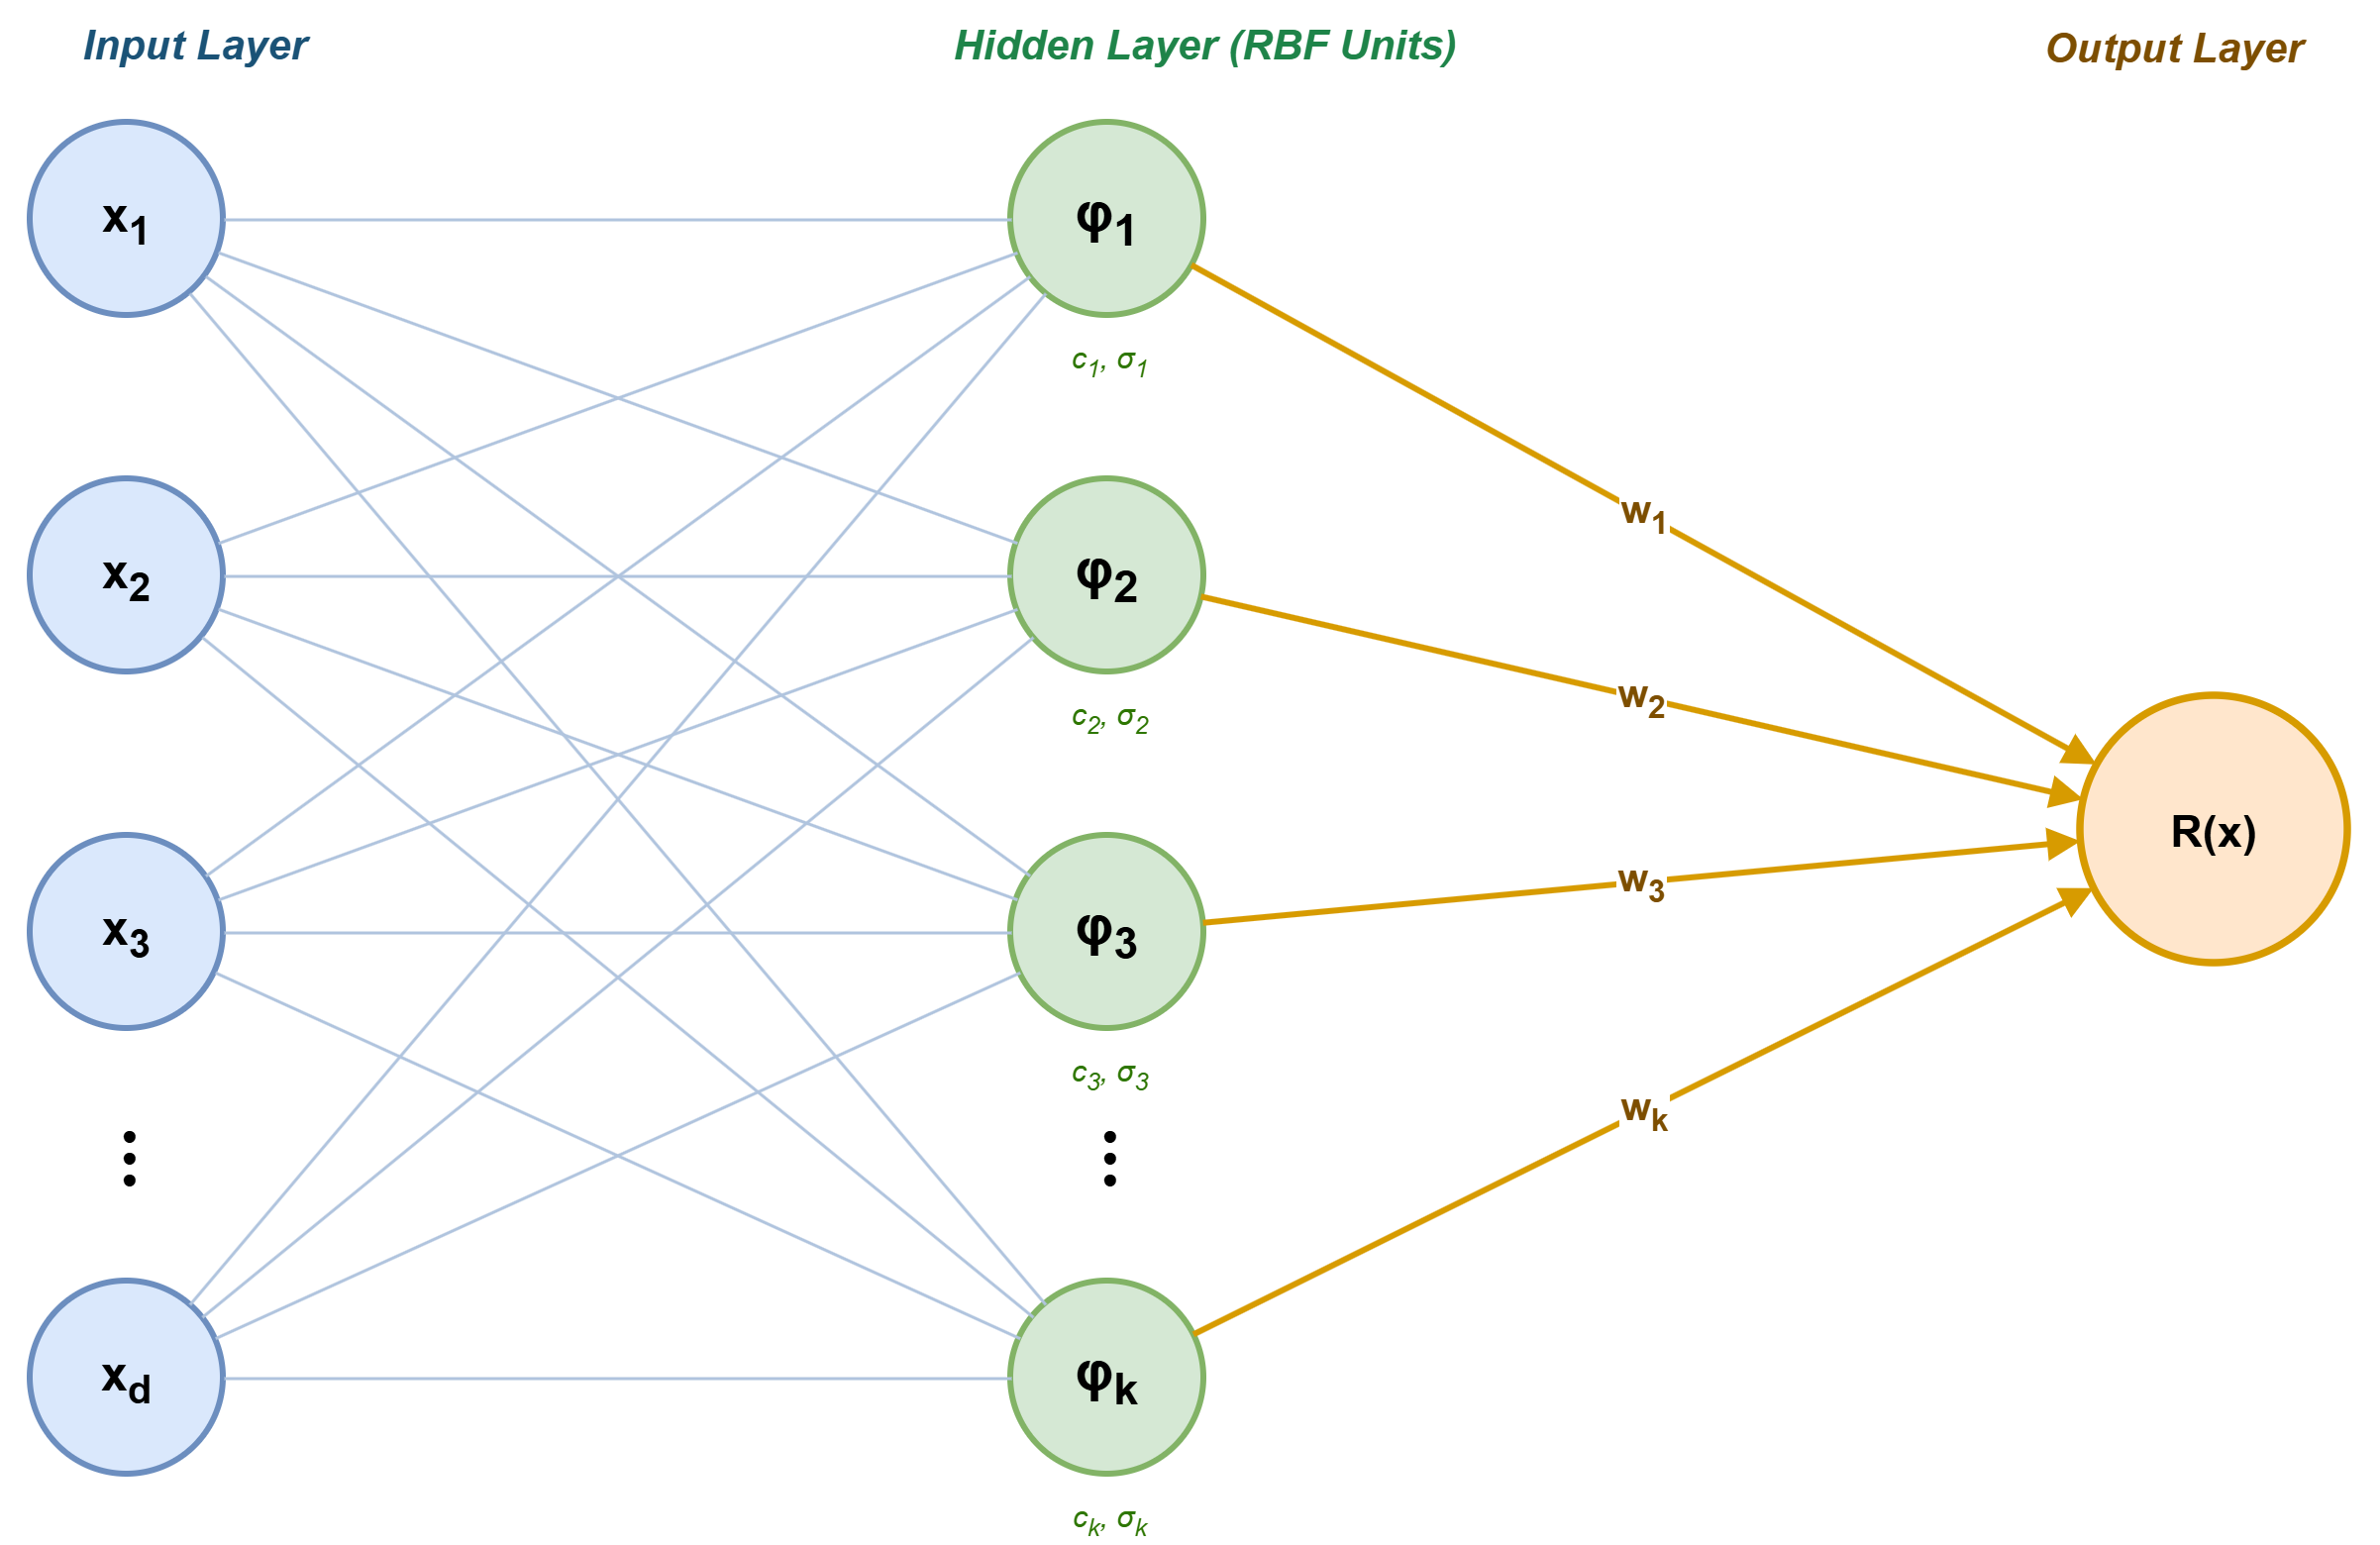
\includegraphics[scale=0.5]{rbf_network_architecture}
\par\end{centering}
\caption{General structure of an RBF network. The input vector $x$ = ($x_{1}$,
$x_{2}$, ..., $x_{d}$) is fed to $k$ hidden units, each characterized
by a center $c_{i}$ (a reference point in the input space) and a
variance $\sigma_{i}$ (the spread of the basis function). The output
$R(x)$ is a weighted sum of the hidden unit responses, with weights
$w_{i}$. }

\end{figure}

The following notation is used in Equation \ref{eq:firstrbf}:
\begin{enumerate}
\item The vector $\overrightarrow{x}$ denotes the input pattern and the
number of elements in this vector is denoted as $d$.
\item The constant $k$ denotes the number of weights for the RBF network.
\item The vectors $\overrightarrow{c_{i}},\ i=1,..,k$ stand for the so
- called center vectors.
\item The vector $\overrightarrow{w}$ represents the weight vector of the
RBF network.
\item The value $R\left(\overrightarrow{x}\right)$ denotes the predicted
value of the network for the input pattern $\overrightarrow{x}$.
\item The function $\phi(x)$ typically is defined as the following Gaussian
function:
\begin{equation}
\phi(x)=\exp\left(-\frac{\left(x-c\right)^{2}}{\sigma^{2}}\right)
\end{equation}
\end{enumerate}
Moreover, the training error associated with any RBF network $R(x)$
is defined as:
\begin{equation}
E\left(R\left(\overrightarrow{x}\right)\right)=\sum_{i=1}^{M}\left(R\left(\overrightarrow{x_{i}}\right)-y_{i}\right)^{2}\label{eq:RbfError}
\end{equation}
In this equation, the set $\left(\overrightarrow{x_{i}},y_{i}\right),\ i=1,...,M$
represents the training set of the objective problem and the values
$y_{i}$ are the actual outputs for any given pattern $\overrightarrow{x_{i}}$.
The effectiveness of RBF networks has been demonstrated across numerous
application domains. Representative examples include physics-related
problems \citep{rbfphysics1,rbfphysics2,rbfphysics3,rbfphysics4},
differential equation solving \citep{rbfde1,rbfde2,rbfde3}, robotic
systems \citep{rbfrobotics1,rbfrobotics2}, facial recognition \citep{rbfface1},
digital communication systems \citep{rbfnetwork1,rbfnetwork2}, chemical
applications \citep{rbfchemistry1,rbfchemistry2}, economic modeling
\citep{rbfecon0,rbfecon1,rbfecon2}, cybersecurity and network security
tasks \citep{rbf_dos1,rbf_dos2}, time-series forecasting \citep{rbf_time},
and wind energy production prediction \citep{rbf_wind}.

In recent years, numerous studies have introduced novel approaches
for initializing the parameters of RBF networks \citep{rbfinit1,rbfinit2,rbfinit3}.
In addition, the influence of kernel widths on the performance of
RBF networks has been extensively investigated by Benoudjit et al.
\citep{rbfkernel}, while Neruda et al. \citep{rbflearn} provided
a comparative evaluation of several learning algorithms designed for
RBF training. Furthermore, a variety of pruning strategies have been
proposed \citep{rbfprun1,rbfprun3,rbfprun2} with the objective of
reducing the number of network parameters and, consequently, the overall
model complexity. Given the widespread adoption of RBF networks and
the substantial computational effort often required for their training,
several studies have recently focused on exploiting parallel computing
architectures to accelerate neural network parameter optimization
\citep{rbfpar1,rbfpar2}. Finally, Park et al. \citep{rbf_universal}
demonstrated that an RBF network consisting of a single hidden processing
layer possesses the universal approximation property, being capable
of approximating any continuous function with arbitrary accuracy.

In conventional RBF network training, the centers of the basis functions
$\phi(x)$ are initially determined, and the corresponding weight
vector $\overrightarrow{w}$ is subsequently obtained by solving a
linear system of equations. The k-means clustering algorithm \citep{kmeans}
is among the most frequently employed techniques for center selection.
Despite its simplicity and computational efficiency, this approach
often suffers from overfitting, reducing the predictive performance
of the model on unseen samples. Moreover, because the optimization
process does not impose explicit constraints on the parameter values,
the resulting estimates may become excessively large or small, adversely
affecting both model stability and generalization capability.

The present work introduces a novel training methodology for RBF networks
consisting of two distinct phases. During the first phase, a promising
range of values for the network centers and variances is estimated
by exploiting the k-means clustering technique. In the second phase,
a modified genetic algorithm \citep{ga1,ga2} is employed to determine
the optimal values of the centers and variances within the search
intervals identified during the first phase. The weights of the RBF
network are computed through the solution of an appropriate linear
system of equations.

The remaining of this article is organized as follows: in section
\ref{sec:Materials-and-Methods} the proposed method is fully described,
in section \ref{sec:Results} the experimental results are outlined
and finally in section \ref{sec:Conclusions} a discussion is provided
on the experimental results.

\section{Materials and Methods\label{sec:Materials-and-Methods}}

\subsection{The first phase of the proposed method}

In the first phase, the k-means clustering algorithm is employed to
estimate promising search intervals for the centers and variances
of the RBF network. Specifically, for each network parameter, the
corresponding search interval is defined as a multiple of the value
produced by the k-means algorithm, thereby providing a bounded region
for the subsequent optimization process. The k-means algorithm is
presented in Algorithm \ref{alg:KMEANS}.

\begin{algorithm}[H]
\caption{The k-means algorithm used to estimate centers and variances.\label{alg:KMEANS}}

\begin{enumerate}
\item \textbf{Initialization}
\begin{enumerate}
\item \textbf{Input}: the train set $\left(\overrightarrow{x_{i}},y_{i}\right),\ i=1,...,M$
of the objective problem.
\item \textbf{Set} as $k$ the number of desired centers.
\item \textbf{Initialize} the set $S_{j}=\{\ \}$, $j=1,\ldots,k$.
\end{enumerate}
\item \textbf{Repeat}
\begin{enumerate}
\item \textbf{For} $i=1,\ldots,M$ \textbf{do}
\begin{enumerate}
\item \textbf{Set} $j^{*}=\mbox{argmin}_{m=1}^{k}\left\{ D\left(x_{i},c_{m}\right)\right\} $.
In this formulation, $j^{*}$ denotes the index of the closest center
to the input sample $\overrightarrow{x_{i}}$, whereas $D(x,y)$ corresponds
to the Euclidean distance function.
\item \textbf{Set} $S_{j^{*}}=S_{j^{*}}\cup\left\{ x_{i}\right\} $.
\end{enumerate}
\item \textbf{End For}
\item \textbf{For} $j=1..k$ \textbf{do}
\begin{enumerate}
\item \textbf{Calculate} the number of points in each cluster $S_{j}$ and
denote them as $M_{j}$.
\item \textbf{Calculate }every center $\overrightarrow{c_{i}}$ using the
equation:
\[
\overrightarrow{c_{i}}=\frac{1}{M_{j}}\sum_{x_{i}\in S_{j}}x_{i}
\]
\end{enumerate}
\item \textbf{End} \textbf{For}
\end{enumerate}
\item \textbf{If} the centers $\overrightarrow{c_{i}},j=1,\ldots,k$ did
not change then the loop is terminated.
\item \textbf{End Repeat}
\item The algorithm \textbf{returns} as output the estimated centers $\overrightarrow{c_{i}},\ i=1,..,k$
and the associated variances $\sigma_{i},\ i=1,\ldots,k$
\end{enumerate}
\end{algorithm}
The set of parameters comprising the centers and variances of an RBF
network with $k$ hidden units is represented by a vector of dimension
\begin{equation}
n=k\times d+d\label{eq:nparams}
\end{equation}
 where $d$ denotes the dimensionality of the input patterns. This
vector has the following structure:
\begin{equation}
\overrightarrow{I}=\left\{ c_{11},c_{12},c_{1d},\sigma_{1},c_{21},c_{22},\ldots,c_{2d},\sigma_{2},\ldots,c_{k1},c_{k2},\ldots,c_{kd},\sigma_{k}\right\} \label{eq:ixstructure}
\end{equation}
For this vector of parameters the bound vectors $\overrightarrow{L},\ \overrightarrow{R}$
are constructed using the procedure depicted in Algorithm \ref{alg:boundVectors}.

\begin{algorithm}[H]
\caption{The algorithm that is used to construct the bound vectors $\protect\overrightarrow{L},\ \protect\overrightarrow{R}$.\label{alg:boundVectors}}

\begin{enumerate}
\item \textbf{Input}: the vector $\overrightarrow{I}$ of Equation \ref{eq:ixstructure}.
\item \textbf{Input}: the scale factor used for the bound vectors denoted
as $F$ with $F\ge1$.
\item \textbf{Input}: a small positive number $v_{e}$ used as the low limit
of the variables representing the variances of the RBF network.
\item \textbf{Set} $m=1$
\item \textbf{For} $i=1,\ldots,k$ \textbf{do}
\begin{enumerate}
\item \textbf{For} $j=1,\ldots,d$ \textbf{do }//this loop is for the variables
of each center
\begin{enumerate}
\item \textbf{Set} $L_{m}=-F\times I_{m}$
\item \textbf{Set} $R_{m}=F\times I_{m}$
\item \textbf{Set} $m=m+1$
\end{enumerate}
\item \textbf{End For}
\item \textbf{Set} $L_{m}=v_{e}$ //set the bounds for the variables representing
the variances.
\item \textbf{Set} $R_{m}=F\times I_{m}$
\item \textbf{Set} $m=m+1$
\end{enumerate}
\item \textbf{End For}
\item \textbf{Output}: The bound vectors $\overrightarrow{L},\ \overrightarrow{R}$
\end{enumerate}
\end{algorithm}


\subsection{The description of the second phase}

In the second phase of the proposed algorithm, a genetic algorithm
is employed to optimize the centers and variances of the RBF network
within the search intervals defined by the vectors $\overrightarrow{L},\ \overrightarrow{R}$
obtained during the first phase. The output weight vector $\overrightarrow{w}$
of the RBF network is subsequently computed by solving the corresponding
linear system of equations. Within the proposed genetic algorithm,
each chromosome follows the structure of the parameter vector $\overrightarrow{I}$
introduced in Equation \ref{eq:ixstructure}, where all decision variables
corresponding to the RBF centers and variances are encoded. 

A suitably modified genetic algorithm was adopted in this stage because
genetic algorithms constitute robust evolutionary optimization techniques
that have demonstrated their effectiveness across a broad spectrum
of practical applications. In addition, they are particularly well
suited for integration with machine learning models, as they generally
require only the formulation of a suitable fitness function while
treating the underlying model as a black-box optimization problem.
For example they have been applied to energy problems \citep{gen_app1},
water distribution problems \citep{gen_app2}, economic problems \citep{gen_app3},
training of of neural networks \citep{gen_app4} etc. The steps of
the used genetic algorithm have as follows:
\begin{enumerate}
\item \textbf{Initialization step}. 
\begin{enumerate}
\item The algorithm has the following set of parameters:
\begin{enumerate}
\item $N_{c}$, the desired number of chromosomes.
\item $N_{g}$, the maximum number of allowed generations.
\item $p_{s}$, the used selection rate with $p_{s}\le1$.
\item $p_{m},$ the used mutation rate with $p_{m}\le1$.
\end{enumerate}
\item \textbf{Construct} a set of chromosomes with dimension $n$ as defined
in Equation \ref{eq:nparams}. Each chromosome represents the centers
and variances of any given RBF network and the value of each chromosome
is initialized inside the bound vectors $\overrightarrow{L},\ \overrightarrow{R}$.
\item \textbf{Set} $k=0$, which represents the current number of generations.
\end{enumerate}
\item \textbf{Fitness calculation step}.
\begin{enumerate}
\item \textbf{For} $i=1,\ldots,N_{c}$ \textbf{do}
\begin{enumerate}
\item \textbf{Produce }an RBF network $R_{i}=R\left(\overrightarrow{x},\overrightarrow{g_{i}}\right).$
The centers and variances of $R_{i}$ are derived from chromosome
$\overrightarrow{g_{i}}$. The weight vector $\overrightarrow{w}=\left(w_{1},w_{2},\ldots,w_{k}\right)$
is calculated as follows: 
\begin{enumerate}
\item \textbf{Set} \textbf{$W=w_{kj}$}
\item \textbf{Set} \textbf{$\Phi=\phi_{j}\left(x_{i}\right)$}, that denotes
the outputs of the computation units.
\item \textbf{Set $T=\left\{ t_{i}=y_{i},i=1,..,M\right\} $}, that denotes
the real outputs for the training set.
\item \textbf{Solve }the following system of equations:\textbf{ }
\begin{equation}
\Phi^{T}\left(T-\Phi W^{T}\right)=0
\end{equation}
The solution is:
\begin{equation}
W^{T}=\left(\Phi^{T}\Phi\right)^{-1}\Phi^{T}T=\Phi^{\dagger}T\label{eq:eqoutput}
\end{equation}
\end{enumerate}
\item \textbf{Calculate} the corresponding fitness value $f_{i}$ as
\begin{equation}
f_{i}=\sum_{j=1}^{M}\left(R\left(\overrightarrow{x}_{j},\overrightarrow{g_{i}}\right)-y_{j}\right)^{2}\label{eq:eq1-1}
\end{equation}
\end{enumerate}
\item \textbf{End For}
\end{enumerate}
\item \textbf{Genetic operations step}.
\begin{enumerate}
\item \textbf{Selection} procedure: The population is first ordered based
on fitness. A fraction $p_{s}$ of the population, corresponding to
the top $p_{s}\times N_{c}$ chromosomes, is retained intact for the
next generation. The rest of the population is regenerated by applying
crossover and mutation operations to selected parent chromosomes.
\item \textbf{Crossover} procedure: In this step $\left(1-p_{s}\right)\times N_{c}$
new offsprings will be produced. For each pair $\left(\tilde{z},\tilde{w}\right)$
of these new chromosomes, two chromosomes $(z,w)$ are chosen from
the current population with the assistance of tournament selection.
The new chromosomes will be created using the following equations:
\begin{eqnarray}
\tilde{z_{i}} & = & a_{i}z_{i}+\left(1-a_{i}\right)w_{i}\nonumber \\
\tilde{w_{i}} & = & a_{i}w_{i}+\left(1-a_{i}\right)z_{i}\label{eq:crossover_ali-1}
\end{eqnarray}
In this equation the $a_{i}$ denote random numbers in the range $[-0.5,1.5]$
\citep{kaelo}. 
\item \textbf{Mutation} procedure: Select a random number $r\in[0,1]$ for
each element $\overrightarrow{g_{i,j}},j=1,\ldots,n$ for the corresponding
chromosome $g_{i}$ . If $r\le p_{m}$ , then this element is changed
using the following scheme:
\end{enumerate}
\begin{equation}
\overrightarrow{g_{i,j}}=\overrightarrow{g_{i,j}}+t\times p_{c}\times\overrightarrow{g_{i,j}}\label{eq:mutation}
\end{equation}
where $p_{c}$ is a number in range $[0,1]$ that denotes the magnitude
of changes applied to the current element and $t$ is randomly selected
integer that could be $-1$ or $1$.
\item \textbf{Termination check step}.
\begin{enumerate}
\item \textbf{Set} $k=k+1$
\item \textbf{If} $k<N_{g}$then \textbf{goto} Fitness Calculation step.
\item \textbf{Otherwise, }obtain the best chromosome $\overrightarrow{g^{*}}$
and create the associated RBF network $R^{*}=R\left(\overrightarrow{x},\overrightarrow{g^{*}}\right)$.
The weight vector for this RBF network is also obtained by solving
a similar system of equations as in Fitness Calculation Step.
\item \textbf{Apply} a local search procedure to minimize the error function:
\begin{equation}
f^{*}=\sum_{j=1}^{M}\left(R^{*}\left(\overrightarrow{x}_{j},\overrightarrow{g^{*}}\right)-y_{j}\right)^{2}\label{eq:eq1-1-1}
\end{equation}
A modified BFGS algorithm based on the method of Powell \citep{powell}
was adopted as the local optimization procedure. This variant efficiently
enforces the parameter bounds established during the preceding stage
of the proposed methodology.
\end{enumerate}
\end{enumerate}
\medskip{}

The overall structure of the second phase is illustrated in Figure
\ref{fig:FlowchartSecondPhase}. The procedure begins with the initialization
of a population of chromosomes within the parameter bounds established
during the first phase. The centers and variances of each candidate
RBF network are extracted directly from the corresponding chromosome,
the network weights are subsequently estimated by solving the corresponding
linear system of equations, and a fitness value is assigned to each
candidate based on the resulting prediction error. Following the evaluation
of all candidates, the genetic operations of selection, crossover,
and mutation are applied to produce the next generation. The generation
counter is then incremented and checked against the maximum allowed
number of generations. This cycle repeats until the termination criterion
is met. At that point, the best chromosome identified throughout the
search is used to reconstruct the final RBF network, whose weights
are re-estimated by solving the linear system once more, after which
a local optimization step based on the BFGS method is applied to further
refine the solution.

\begin{figure}[H]

\begin{centering}
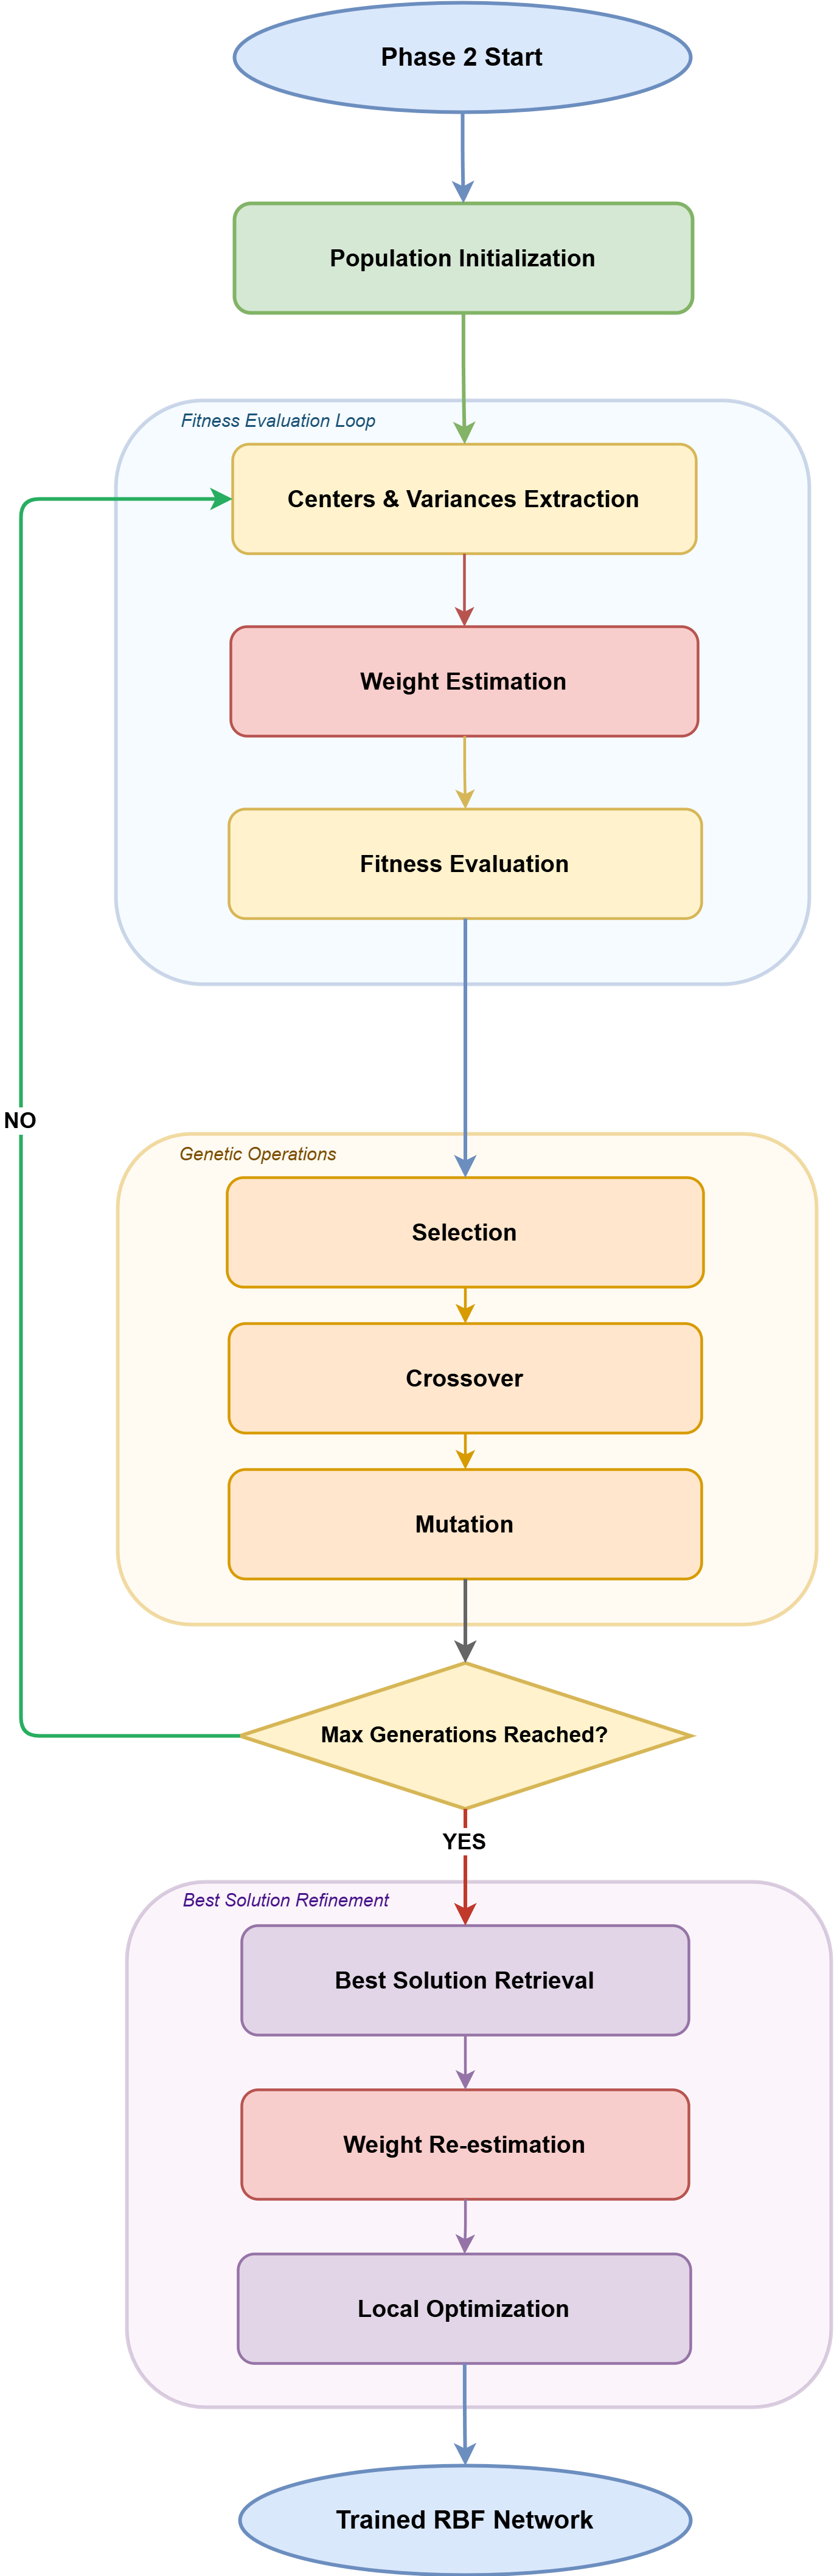
\includegraphics[scale=0.5]{rbf_phase2_flowchart}
\par\end{centering}
\caption{Flowchart of the second phase of the proposed training procedure.\label{fig:FlowchartSecondPhase}}
\end{figure}


\section{Results\label{sec:Results}}

\subsection{Experimental datasets The datasets used in the conducted experiments
were obtained from the following online databases:}
\begin{enumerate}
\item The UCI website, \url{https://archive.ics.uci.edu/}(accessed on 24
June 2026)\citep{uci}
\item The Keel website, \url{https://sci2s.ugr.es/keel/datasets.php}(accessed
on 24 June 2026)\citep{Keel}.
\item The Statlib URL \url{ftp://lib.stat.cmu.edu/datasets/index.html }(accessed
on 24 June 2026). 
\end{enumerate}
The list of classification datasets has as follows:
\begin{enumerate}
\item \textbf{Appendictis} dataset, which is a medical dataset\citep{appendicitis}.
\item \textbf{Alcohol} dataset, related to alcohol consumption and appeared
in \citep{alcohol}. 
\item \textbf{Australian} dataset \citep{australian} used in economics.
\item \textbf{Balance} dataset \citep{balance}, related to various psychological
experiments. 
\item \textbf{Bands} dataset, used to detect printing problems \citep{Bands}.
\item \textbf{Circular} dataset, which is produced artificially and contains
two distinct classes.
\item \textbf{Cleveland} dataset, related to the presence of heart disease
\citep{cleveland1,cleveland2}.
\item \textbf{Dermatology} dataset \citep{dermatology}, a medical dataset.
\item \textbf{Ecoli}, used to detect protein problems \citep{ecoli}.
\item The \textbf{Fert} dataset, related to sperm concentration problems.
\item \textbf{Glass} dataset, related to glass issues.
\item \textbf{Haberman}, a medical dataset that contains data used in the
prediction of breast cancer.
\item \textbf{Hayes roth} dataset\citep{hayesroth}.
\item \textbf{Heart} dataset \citep{heart}, which was used to detect heart
diseases.
\item \textbf{HeartAttack}, a medical dataset related to heart diseases
\item \textbf{HouseVotes} dataset \citep{housevotes}.
\item \textbf{Ionosphere} dataset, that was used to classify radar data
from the ionosphere \citep{ion1,ion2}.
\item \textbf{Liverdisorder} dataset \citep{liver}, which is a medical
dataset.
\item \textbf{Lymography} dataset\citep{lymography}.
\item \textbf{Mammographic} dataset \citep{mammographic}, which is a medical
dataset related to breast tumors.
\item \textbf{Parkinsons} dataset, which is a medical dataset used to detect
the presence of the Parkinson's Disease\citep{parkinsons}.
\item \textbf{Page Blocks} dataset, related to the determination of blocks
inside various documents.
\item \textbf{Phoneme}, a dataset related to sound.
\item \textbf{Pima} dataset, which is a medical dataset used widely \citep{pima}.
\item \textbf{Popfailures} dataset \citep{popfailures}, used in various
experiments regarding climate.
\item \textbf{Ring}, a dataset related to some distributions. 
\item \textbf{Spiral} dataset, which was produced artificially and contains
two classes.
\item \textbf{Regions2} dataset \citep{regions}. 
\item \textbf{Saheart} dataset \citep{saheart}, a medical dataset related
to the presence of heart diseases. 
\item \textbf{Satimage} dataset, related to satellite images.
\item \textbf{Segment} dataset \citep{segment}, which is an image processing
dataset.
\item The \textbf{Sonar} dataset \citep{sonar}.
\item \textbf{Spambase }dataset, regarding the detection of spam emails
\citep{spambase}. 
\item \textbf{Statheart}, which is medical dataset on heart diseases.
\item \textbf{Student}, which contains data from various experiments in
schools \citep{student}.
\item \textbf{Transfusion} dataset \citep{transfusion}.
\item \textbf{Wdbc} dataset \citep{wdbc}, which is a medical dataset related
the presence of breast tumors. 
\item \textbf{Wine} dataset, used for the classification of the quality
of wines  \citep{wine1,wine2}.
\item \textbf{Eeg} dataset, which is an EEG dataset \citep{eeg} . From
this dataset the following cases were used: Z\_F\_S, ZONF\_S and ZO\_NF\_S.
\item \textbf{Zoo} dataset \citep{zoo}, which was used to estimate the
class of various animals.
\end{enumerate}
In addition, the list of the used regression datasets has as follows:
\begin{enumerate}
\item \textbf{Abalone}, used to detect the age of abalones \citep{abalone}.
\item \textbf{Airfoil}, a dataset derived from NASA \citep{airfoil}.
\item \textbf{Auto}, used to estimate the fuel consumption of cars.
\item \textbf{BK}, used to estimate the points scored in basketball games. 
\item \textbf{BL}, that contains measurements from electricity experiments.
\item \textbf{Baseball}, used for the estimation of income of baseball players.
\item \textbf{Concrete}, a dataset that contains data from civil engineering
\citep{concrete}.
\item \textbf{DEE}, a dataset related to the prediction of the prices of
electricity. 
\item \textbf{FY, }that contains measurements related to fruit flies. 
\item \textbf{HO}, which was downloaded from the STATLIB repository.
\item \textbf{Housing}, a dataset that contains data from prices of houses
\citep{housing}.
\item \textbf{Laser}, a dataset containing data from various physics experiments.
\item \textbf{LW}, a dataset used to detect problems in the weight of babes.
\item \textbf{MB} dataset \citep{key21}.
\item \textbf{Mortgage}, a dataset that contains economic data.
\item \textbf{NT} dataset\citep{ntdataset}. 
\item \textbf{PL} dataset, which was downloaded from the STATLIB repository.
\item \textbf{Plastic}, a dataset that contains measurements from plastic
experiments.
\item \textbf{PY} dataset\citep{pydataset}. 
\item \textbf{Quake}, related to measurements on quakes.
\item \textbf{SN}, which is a benchmark dataset obtained from the STATLIB
repository.
\item \textbf{Stock}, related to the prices of stocks.
\item \textbf{Treasury}, which is a dataset contains economic data.
\item The \textbf{VE} dataset, which was downloaded from the STATLIB repository.
\end{enumerate}

\subsection{Experimental details}

The RBF network implemented in this study was developed in ANSI C++
with the support of the open-source Armadillo library \citep{armadillo}.
The optimization algorithms used were obtained from the OPTIMUS environment,
downloaded from \url{https://github.com/itsoulos/OPTIMUS/}(accessed
on 24 June 2026)\citep{optimus}. Furthermore, derivative computations
required by the optimization procedures were performed using the Adept
automatic differentiation library \citep{adept}. To assess the performance
and generalization capability of the proposed approach, a 10-fold
cross-validation protocol was applied to all datasets. Each experimental
setup was repeated 30 independent times, with a distinct initialization
seed assigned to the random number generator in every run. Random
number generation was carried out using the drand48() function provided
by the C programming language. The average classification error is
defined as: 
\begin{equation}
E_{C}\left(N\left(\overrightarrow{x},\overrightarrow{w}\right)\right)=100\times\frac{\sum_{i=1}^{N}\left(\mbox{class}\left(N\left(\overrightarrow{x_{i}},\overrightarrow{w}\right)\right)-y_{i}\right)}{N}
\end{equation}
The set $T$ denotes the corresponding test set, with $T=\left(x_{i},y_{i}\right),\ i=1,\ldots,N$.
Also, the average regression error is defined as follows:
\begin{equation}
E_{R}\left(N\left(\overrightarrow{x},\overrightarrow{w}\right)\right)=\frac{\sum_{i=1}^{N}\left(N\left(\overrightarrow{x_{i}},\overrightarrow{w}\right)-y_{i}\right)^{2}}{N}
\end{equation}

The settings used in the conducted experiments are listed in Table
\ref{tab:Experimental-settings.}. 
\begin{table}[H]
\caption{Experimental settings.\label{tab:Experimental-settings.}}

\centering{}%
\begin{tabular}{|c|c|c|}
\hline 
PARAMETER & MEANING & VALUE\tabularnewline
\hline 
\hline 
$N_{c}$ & \begin{cellvarwidth}[t]
\centering
Number of \\
chromosomes
\end{cellvarwidth} & 500\tabularnewline
\hline 
$N_{g}$ & \begin{cellvarwidth}[t]
\centering
Maximum number\\
of generations
\end{cellvarwidth} & 500\tabularnewline
\hline 
$p_{s}$ & Selection rate & 0.10\tabularnewline
\hline 
$p_{m}$ & Mutation rate & 0.05\tabularnewline
\hline 
$p_{c}$ & Mutation magnitude & 0.05\tabularnewline
\hline 
$F$ & Scale factor & 4.0\tabularnewline
\hline 
$v_{e}$ & \begin{cellvarwidth}[t]
\centering
Small value\\
used in variances
\end{cellvarwidth} & 0.01\tabularnewline
\hline 
$k$ & Number of weights & 10\tabularnewline
\hline 
\end{tabular}
\end{table}
Also, in the tables containing experimental results the following
notation is used:
\begin{enumerate}
\item The column DATASET represents the name of the used dataset.
\item The column BFGS stands for the results obtained when the BFGS optimization
procedure \citep{bfgs} is used to train an artificial neural network
\citep{nn1,nn2} with 10 processing nodes.
\item The ADAM column stands for the usage of the ADAM optimizer \citep{Adam,AdamNN}
to train a neural network with 10 processing nodes.
\item The column RBF represents the results where the traditional training
method is used to train an RBF network with 10 processing nodes.
\item The column NEAT \citep{neat} is used to denote the results from NEAT
(NeuroEvolution of Augmenting Topologies).
\item The column GRBF is used for the experimental results of the method
presented in \citep{genrbf} to train an RBF network with 10 processing
nodes.
\item The column PROPOSED stands for the results obtained by the incorporation
of the proposed method.
\item The row labeled AVERAGE presents the mean classification or regression
error obtained across the entire collection of datasets.
\end{enumerate}

\subsection{Comparison with other machine learning methods}

The results of the comparative evaluation are presented in Table \ref{tab:experClass}
for the classification problems and in Table \ref{tab:experRegression}
for the regression problems, while Figures \ref{fig:classMethods}
and \ref{fig:regressionMethods} display the distribution of errors
via box plots and report the outcomes of the overall Friedman test.
For classification tasks (Table \ref{tab:experClass}), the mean error
rates were 35.18\% for ADAM, 35.50\% for GRBF, 33.25\% for BFGS, 32.16\%
for NEAT, 28.68\% for RBF, and 21.58\% for the Proposed method. The
overall Friedman test (Figure \ref{fig:classMethods}) yielded $p=4.5\times10^{-10}$,
confirming that the differences among methods are statistically significant
at a very high confidence level. The Proposed method achieves the
lowest mean error and outperforms the second-best method, RBF, by
approximately 24.8\%. At the individual dataset level, the Proposed
method ranked first in 26 out of 42 datasets (61.9\%), with particularly
strong performance on RING, SPAMBASE, Z\_F\_S, and ZONF\_S, as detailed
in Table \ref{tab:experClass}.

\begin{table}[H]
\caption{Experimental results on the classification datasets, using a variety
of machine learning methods.\label{tab:experClass}}

\centering{}%
\begin{tabular}{|c|c|c|c|c|c|c|}
\hline 
DATASET & ADAM & BFGS & NEAT & RBF & GRBF & PROPOSED\tabularnewline
\hline 
\hline 
APPENDICITIS & 16.50\% & 18.00\% & 17.20\% & 12.23\% & 16.83\% & 17.80\%\tabularnewline
\hline 
ALCOHOL & 57.78\% & 41.50\% & 66.80\% & 49.38\% & 52.45\% & 20.43\%\tabularnewline
\hline 
AUSTRALIAN & 35.65\% & 38.13\% & 31.98\% & 34.89\% & 41.79\% & 18.90\%\tabularnewline
\hline 
BALANCE & 12.27\% & 8.64\% & 23.14\% & 33.53\% & 38.02\% & 17.50\%\tabularnewline
\hline 
BANDS & 36.92\% & 36.67\% & 34.30\% & 37.17\% & 43.95\% & 36.28\%\tabularnewline
\hline 
CIRCULAR & 19.95\% & 6.08\% & 35.18\% & 5.98\% & 21.43\% & 5.04\%\tabularnewline
\hline 
CLEVELAND & 67.55\% & 77.55\% & 53.44\% & 67.10\% & 67.47\% & 50.14\%\tabularnewline
\hline 
DERMATOLOGY & 26.14\% & 52.92\% & 32.43\% & 62.34\% & 61.46\% & 39.80\%\tabularnewline
\hline 
ECOLI & 64.43\% & 69.52\% & 43.44\% & 59.48\% & 70.58\% & 58.36\%\tabularnewline
\hline 
FERT & 23.98\% & 23.20\% & 15.37\% & 15.00\% & 15.00\% & 21.40\%\tabularnewline
\hline 
GLASS & 61.38\% & 54.67\% & 55.71\% & 50.05\% & 66.91\% & 52.76\%\tabularnewline
\hline 
HABERMAN & 29.00\% & 29.34\% & 24.04\% & 25.10\% & 24.37\% & 27.37\%\tabularnewline
\hline 
HAYES ROTH & 59.70\% & 37.33\% & 50.15\% & 64.36\% & 63.46\% & 40.08\%\tabularnewline
\hline 
HEART & 38.53\% & 39.44\% & 39.27\% & 31.20\% & 28.44\% & 22.00\%\tabularnewline
\hline 
HEARTATTACK & 45.55\% & 46.67\% & 32.34\% & 29.00\% & 40.48\% & 19.13\%\tabularnewline
\hline 
HOUSEVOTES & 7.48\% & 7.13\% & 10.89\% & 6.13\% & 11.99\% & 4.61\%\tabularnewline
\hline 
IONOSPHERE & 16.64\% & 15.29\% & 19.67\% & 16.22\% & 19.83\% & 12.83\%\tabularnewline
\hline 
LIVERDISORDER & 41.53\% & 42.59\% & 30.67\% & 30.84\% & 36.97\% & 30.41\%\tabularnewline
\hline 
LYMOGRAPHY & 39.79\% & 35.43\% & 33.70\% & 25.50\% & 29.33\% & 24.57\%\tabularnewline
\hline 
MAMMOGRAPHIC & 46.25\% & 17.24\% & 22.85\% & 21.38\% & 30.41\% & 17.72\%\tabularnewline
\hline 
PARKINSONS & 24.06\% & 27.58\% & 18.56\% & 17.41\% & 33.81\% & 15.53\%\tabularnewline
\hline 
PAGE BLOCKS & 34.27\% & 8.49\% & 10.22\% & 10.09\% & 10.83\% & 9.47\%\tabularnewline
\hline 
PHONEME & 29.43\% & 15.58\% & 22.34\% & 23.32\% & 27.70\% & 15.59\%\tabularnewline
\hline 
PIMA & 34.85\% & 35.59\% & 34.51\% & 25.78\% & 27.83\% & 23.59\%\tabularnewline
\hline 
POPFAILURES & 5.18\% & 5.24\% & 7.05\% & 7.04\% & 7.08\% & 5.61\%\tabularnewline
\hline 
REGIONS2 & 29.85\% & 36.28\% & 33.23\% & 38.29\% & 39.98\% & 25.71\%\tabularnewline
\hline 
RING & 28.80\% & 29.44\% & 30.85\% & 21.67\% & 52.03\% & 5.05\%\tabularnewline
\hline 
SAHEART & 34.04\% & 37.48\% & 34.51\% & 32.19\% & 33.90\% & 28.89\%\tabularnewline
\hline 
SATIMAGE & 73.22\% & 71.73\% & 76.19\% & 40.19\% & 61.20\% & 32.97\%\tabularnewline
\hline 
SEGMENT & 49.75\% & 68.97\% & 66.72\% & 59.68\% & 54.25\% & 32.47\%\tabularnewline
\hline 
SONAR & 30.33\% & 25.85\% & 34.10\% & 27.90\% & 37.13\% & 24.00\%\tabularnewline
\hline 
SPAMBASE & 48.05\% & 18.16\% & 35.77\% & 29.35\% & 35.36\% & 10.54\%\tabularnewline
\hline 
SPIRAL & 47.67\% & 47.99\% & 48.66\% & 44.87\% & 50.02\% & 41.03\%\tabularnewline
\hline 
STATHEART & 44.04\% & 39.65\% & 44.36\% & 31.36\% & 42.94\% & 23.89\%\tabularnewline
\hline 
STUDENT & 5.13\% & 7.14\% & 10.20\% & 5.49\% & 33.26\% & 12.43\%\tabularnewline
\hline 
TRANSFUSION & 25.68\% & 25.84\% & 24.87\% & 26.41\% & 25.67\% & 25.23\%\tabularnewline
\hline 
WDBC & 35.35\% & 29.91\% & 12.88\% & 7.27\% & 8.82\% & 4.19\%\tabularnewline
\hline 
WINE & 29.40\% & 59.71\% & 25.43\% & 31.41\% & 31.47\% & 10.59\%\tabularnewline
\hline 
Z\_F\_S & 47.81\% & 39.37\% & 38.41\% & 13.16\% & 23.37\% & 4.68\%\tabularnewline
\hline 
ZO\_NF\_S & 47.43\% & 43.04\% & 43.75\% & 9.02\% & 22.18\% & 5.47\%\tabularnewline
\hline 
ZONF\_S & 11.99\% & 15.62\% & 5.44\% & 4.03\% & 17.41\% & 1.82\%\tabularnewline
\hline 
ZOO & 14.13\% & 10.70\% & 20.27\% & 21.93\% & 33.50\% & 10.60\%\tabularnewline
\hline 
\textbf{AVERAGE} & \textbf{35.18\%} & \textbf{33.25\%} & \textbf{32.16\%} & \textbf{28.68\%} & \textbf{35.50\%} & \textbf{21.58\%}\tabularnewline
\hline 
\end{tabular}
\end{table}

\begin{figure}[H]
\begin{centering}

\includegraphics[scale=0.5]{stat_tbl2}
\par\end{centering}
\caption{Classification error distribution across the six evaluated methods
(overall Friedman test: $p=4.5\times10^{-10}$)\label{fig:classMethods}}
\end{figure}

\begin{table}[H]
\caption{Experimental results on the used regression datasets using the series
of machine learning methods.\label{tab:experRegression}}

\centering{}%
\begin{tabular}{|c|c|c|c|c|c|c|}
\hline 
DATASET & ADAM & BFGS & NEAT & RBF & GRBF & PROPOSED\tabularnewline
\hline 
\hline 
ABALONE & 4.30 & 5.69 & 9.88 & 7.37 & 9.98 & 6.37\tabularnewline
\hline 
AIRFOIL & 0.005 & 0.003 & 0.067 & 0.27 & 0.121 & 0.004\tabularnewline
\hline 
AUTO & 70.84 & 60.97 & 56.06 & 17.87 & 16.78 & 10.02\tabularnewline
\hline 
BK & 0.025 & 0.28 & 0.15 & 0.02 & 0.023 & 0.021\tabularnewline
\hline 
BL & 0.622 & 2.55 & 0.05 & 0.013 & 0.005 & 0.0005\tabularnewline
\hline 
BASEBALL & 77.90 & 119.63 & 100.39 & 93.02 & 98.91 & 53.20\tabularnewline
\hline 
CONCRETE & 0.078 & 0.066 & 0.081 & 0.011 & 0.015 & 0.008\tabularnewline
\hline 
DEE & 0.63 & 2.36 & 1.512 & 0.17 & 0.25 & 0.16\tabularnewline
\hline 
FA & 0.048 & 0.426 & 0.19 & 0.015 & 0.15 & 0.019\tabularnewline
\hline 
FY & 0.038 & 0.22 & 0.08 & 0.011 & 0.041 & 0.051\tabularnewline
\hline 
HO & 0.035 & 0.62 & 0.169 & 0.03 & 0.076 & 0.007\tabularnewline
\hline 
HOUSING & 80.998 & 97.38 & 56.49 & 57.68 & 95.69 & 10.36\tabularnewline
\hline 
LASER & 0.03 & 0.015 & 0.084 & 0.03 & 0.075 & 0.0198\tabularnewline
\hline 
LW & 0.028 & 2.98 & 0.17 & 0.03 & 0.057 & 0.016\tabularnewline
\hline 
MB & 0.06 & 0.129 & 0.061 & 5.43 & 0.159 & 0.066\tabularnewline
\hline 
MORTGAGE & 9.24 & 8.23 & 14.11 & 1.45 & 1.92 & 0.0096\tabularnewline
\hline 
NT & 0.006 & 0.129 & 0.027 & 13.97 & 0.01 & 0.006\tabularnewline
\hline 
PLASTIC & 11.71 & 20.32 & 20.77 & 8.62 & 25.91 & 2.30\tabularnewline
\hline 
PY & 0.321 & 0.578 & 0.075 & 0.012 & 0.029 & 0.015\tabularnewline
\hline 
PL & 0.117 & 0.290 & 0.098 & 2.118 & 0.155 & 0.024\tabularnewline
\hline 
QUAKE & 0.039 & 0.012 & 0.102 & 0.01 & 0.79 & 0.036\tabularnewline
\hline 
SN & 0.026 & 0.400 & 0.174 & 0.027 & 0.027 & 0.024\tabularnewline
\hline 
STOCK & 180.893 & 302.43 & 215.818 & 12.23 & 25.18 & 1.208\tabularnewline
\hline 
TREASURY & 11.16 & 9.91 & 15.52 & 2.02 & 1.89 & 0.047\tabularnewline
\hline 
VE & 0.359 & 1.92 & 0.045 & 0.024 & 0.023 & 0.04\tabularnewline
\hline 
\textbf{AVERAGE} & \textbf{17.98} & \textbf{25.50} & \textbf{19.69} & \textbf{8.90} & \textbf{11.13} & \textbf{3.36}\tabularnewline
\hline 
\end{tabular}
\end{table}

\begin{figure}[H]
\begin{centering}

\includegraphics[scale=0.5]{stat_tbl3}
\par\end{centering}
\caption{Regression error distribution for all evaluated methods (overall Friedman
test: $p=1.22\times10^{-6}$).\label{fig:regressionMethods}}
\end{figure}

For regression tasks (Table \ref{tab:experRegression}), the mean
error values were 17.98 for ADAM, 25.50 for BFGS, 19.69 for NEAT,
8.90 for RBF, 11.13 for GRBF, and 3.36 for the Proposed method. The
overall Friedman test (Figure \ref{fig:regressionMethods}) yielded
$p=1.22\times10^{-6}$, again confirming statistically significant
differences across methods. The Proposed method achieves a mean error
of 3.36, representing nearly a threefold improvement over RBF (8.90)
and tenfold over BFGS (25.50). Particularly notable results are observed
on the STOCK dataset (1.208 versus 180.893 for ADAM), HOUSING (10.36
versus 97.38 for BFGS), and MORTGAGE (0.0096 versus 9.24 for ADAM),
as shown in Table \ref{tab:experRegression}.

\subsection{Experiments with the scale parameter $F$ }

Table \ref{tab:experClassF} and Figure \ref{fig:classF} present
the effect of the scale parameter $F$ on classification performance,
while Table \ref{tab:experRegressionF} and Figure \ref{fig:regressionF}
present the corresponding results for regression tasks. For classification
(Table \ref{tab:experClassF}), the mean error rates were 25.93\%
for $F$=1, 22.85\% for $F$=2, 21.58\% for $F$=4, and 21.24\% for
$F$=8. The overall Friedman test (Figure \ref{fig:classF}) yielded
$p=9.36\times10^{-5}$, confirming that the choice of $F$ has a statistically
significant impact on performance. A clear decreasing trend in error
is observed as $F$ increases, with $F$=8 yielding a marginally lower
average than $F$=4. However, the difference between these two settings
is minimal (21.58\% versus 21.24\%), suggesting that $F$=4 represents
a practical default with a favorable performance-to-complexity trade-off.
For regression (Table \ref{tab:experRegressionF}), the mean error
values were 4.69 for $F$=1, 4.03 for $F$=2, 3.36 for $F$=4, and
3.29 for $F$=8, with the Friedman test (Figure \ref{fig:regressionF})
yielding $p=9.06\times10^{-4}$. A consistent improvement is again
observed with increasing $F$, and the results for $F$=4 and $F$=8
are closely comparable across regression datasets.

\begin{table}[H]
\caption{Experimental results on the classification datasets, using the proposed
method and different values for scale parameter $F$.\label{tab:experClassF}}

\centering{}%
\begin{tabular}{|c|c|c|c|c|}
\hline 
DATASET & $F=1$ & $F=2$ & $F=4$ & $F=8$\tabularnewline
\hline 
\hline 
APPENDICITIS & 17.60\% & 14.20\% & 17.80\% & 18.50\%\tabularnewline
\hline 
ALCOHOL & 30.09\% & 23.83\% & 20.43\% & 20.21\%\tabularnewline
\hline 
AUSTRALIAN & 16.35\% & 18.64\% & 18.90\% & 20.13\%\tabularnewline
\hline 
BALANCE & 34.97\% & 23.28\% & 17.50\% & 18.27\%\tabularnewline
\hline 
BANDS & 34.33\% & 35.03\% & 36.28\% & 34.14\%\tabularnewline
\hline 
CIRCULAR & 34.83\% & 8.55\% & 5.04\% & 3.76\%\tabularnewline
\hline 
CLEVELAND & 48.38\% & 49.03\% & 50.14\% & 50.28\%\tabularnewline
\hline 
DERMATOLOGY & 60.10\% & 38.57\% & 39.80\% & 38.26\%\tabularnewline
\hline 
ECOLI & 56.73\% & 59.36\% & 58.36\% & 59.61\%\tabularnewline
\hline 
FERT & 25.80\% & 22.80\% & 21.40\% & 21.70\%\tabularnewline
\hline 
GLASS & 53.90\% & 53.65\% & 52.76\% & 51.29\%\tabularnewline
\hline 
HABERMAN & 28.23\% & 27.24\% & 27.37\% & 27.13\%\tabularnewline
\hline 
HAYES ROTH & 59.69\% & 53.92\% & 40.08\% & 37.31\%\tabularnewline
\hline 
HEART & 22.67\% & 24.15\% & 22.00\% & 20.85\%\tabularnewline
\hline 
HEARTATTACK & 20.03\% & 19.67\% & 19.13\% & 19.17\%\tabularnewline
\hline 
HOUSEVOTES & 5.52\% & 5.26\% & 4.61\% & 5.00\%\tabularnewline
\hline 
IONOSPHERE & 11.20\% & 13.51\% & 12.83\% & 12.43\%\tabularnewline
\hline 
LIVERDISORDER & 30.85\% & 29.65\% & 30.41\% & 29.56\%\tabularnewline
\hline 
LYMOGRAPHY & 32.86\% & 20.50\% & 24.57\% & 23.26\%\tabularnewline
\hline 
MAMMOGRAPHIC & 28.14\% & 21.88\% & 17.72\% & 17.80\%\tabularnewline
\hline 
PARKINSONS & 17.84\% & 17.32\% & 15.53\% & 15.37\%\tabularnewline
\hline 
PAGE BLOCKS & 9.48\% & 9.43\% & 9.47\% & 9.36\%\tabularnewline
\hline 
PHONEME & 23.37\% & 20.32\% & 15.59\% & 15.82\%\tabularnewline
\hline 
PIMA & 23.91\% & 24.87\% & 23.59\% & 23.71\%\tabularnewline
\hline 
POPFAILURES & 10.18\% & 6.43\% & 5.61\% & 5.63\%\tabularnewline
\hline 
REGIONS2 & 25.73\% & 25.97\% & 25.71\% & 25.65\%\tabularnewline
\hline 
RING & 5.55\% & 5.45\% & 5.05\% & 5.57\%\tabularnewline
\hline 
SAHEART & 29.00\% & 29.13\% & 28.89\% & 28.78\%\tabularnewline
\hline 
SATIMAGE & 33.62\% & 34.01\% & 32.97\% & 34.68\%\tabularnewline
\hline 
SEGMENT & 32.05\% & 31.62\% & 32.47\% & 33.33\%\tabularnewline
\hline 
SONAR & 44.05\% & 29.45\% & 24.00\% & 22.05\%\tabularnewline
\hline 
SPAMBASE & 13.39\% & 10.84\% & 10.54\% & 10.44\%\tabularnewline
\hline 
SPIRAL & 36.80\% & 41.27\% & 41.03\% & 41.49\%\tabularnewline
\hline 
STATHEART & 22.74\% & 25.22\% & 23.89\% & 23.26\%\tabularnewline
\hline 
STUDENT & 25.50\% & 19.33\% & 12.43\% & 4.25\%\tabularnewline
\hline 
TRANSFUSION & 25.19\% & 24.92\% & 25.23\% & 24.65\%\tabularnewline
\hline 
WDBC & 4.86\% & 5.19\% & 4.19\% & 4.37\%\tabularnewline
\hline 
WINE & 11.29\% & 9.82\% & 10.59\% & 10.41\%\tabularnewline
\hline 
Z\_F\_S & 5.03\% & 6.80\% & 4.68\% & 5.37\%\tabularnewline
\hline 
ZO\_NF\_S & 5.67\% & 5.74\% & 5.47\% & 7.22\%\tabularnewline
\hline 
ZONF\_S & 2.45\% & 2.22\% & 1.82\% & 2.30\%\tabularnewline
\hline 
ZOO & 29.00\% & 11.80\% & 10.60\% & 9.50\%\tabularnewline
\hline 
\textbf{AVERAGE} & \textbf{25.93\%} & \textbf{22.85\%} & \textbf{21.58\%} & \textbf{21.24\%}\tabularnewline
\hline 
\end{tabular}
\end{table}

\begin{figure}[H]
\begin{centering}
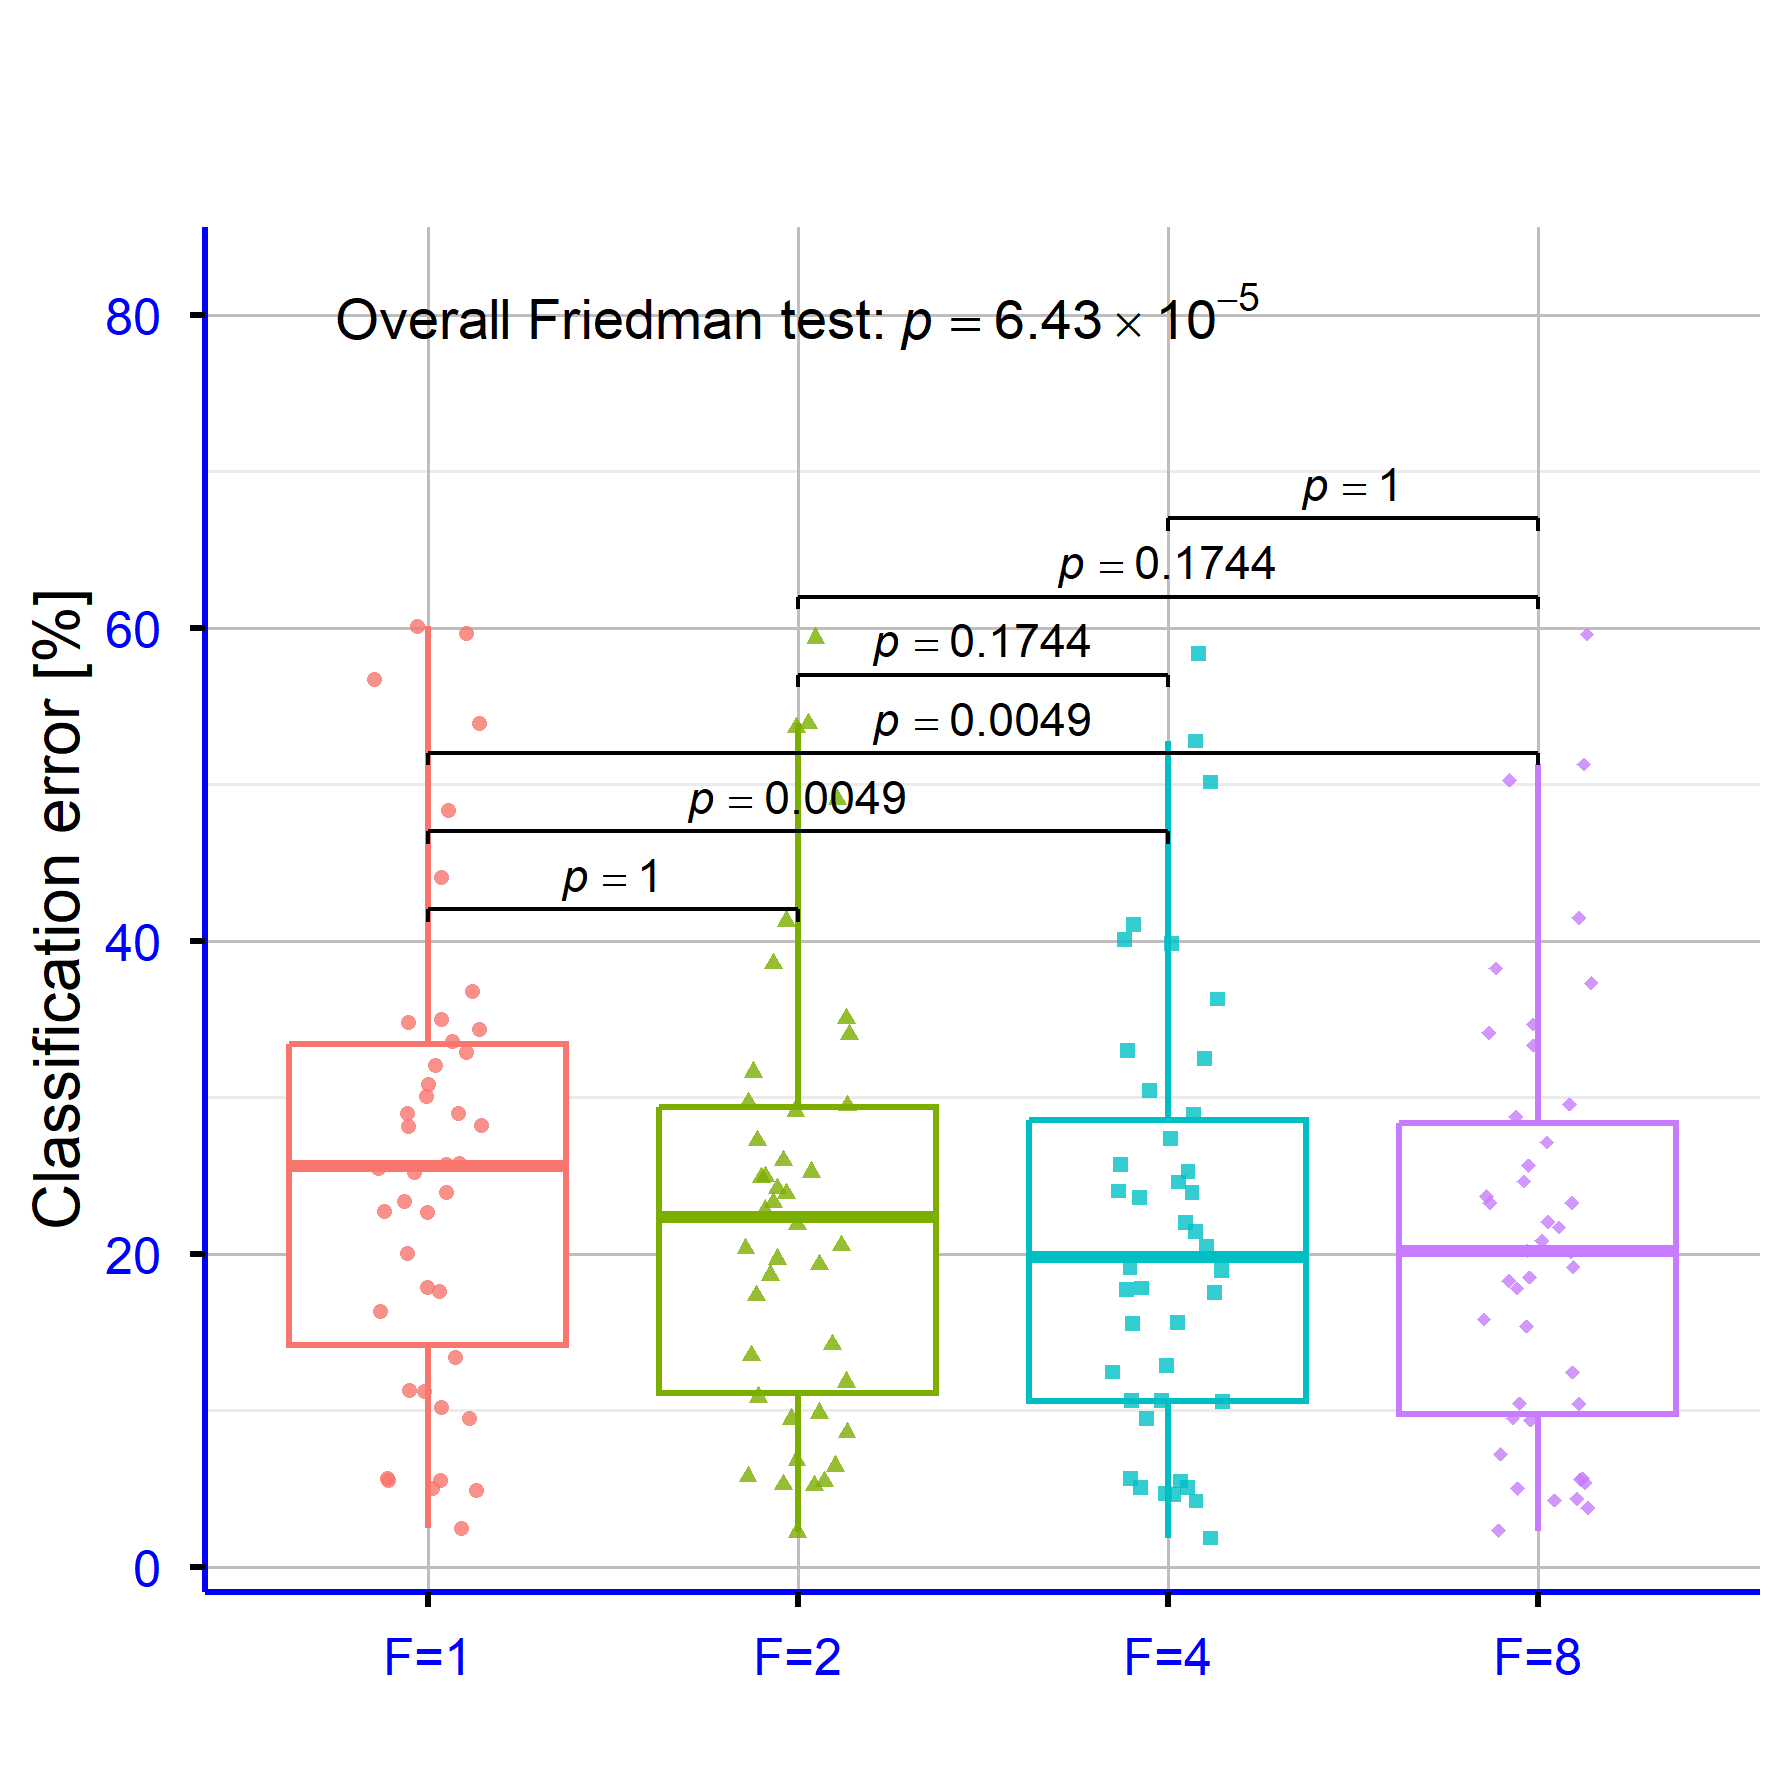
\includegraphics[scale=0.5]{stat_tbl4}
\par\end{centering}
\caption{Effect of the scale parameter F on classification accuracy of the
Proposed method (overall Friedman test: $p=9.36\times10^{-5}$)\label{fig:classF}.}
\end{figure}

\begin{table}[H]
\caption{Experimental results on the used regression datasets using the proposed
method and a series of values for the parameter $F$.\label{tab:experRegressionF}}

\centering{}%
\begin{tabular}{|c|c|c|c|c|}
\hline 
DATASET & $F=1$ & $F=2$ & $F=4$ & $F=8$\tabularnewline
\hline 
\hline 
ABALONE & 10.32 & 7.76 & 6.37 & 5.83\tabularnewline
\hline 
AIRFOIL & 0.004 & 0.004 & 0.004 & 0.004\tabularnewline
\hline 
AUTO & 10.06 & 9.68 & 10.02 & 9.53\tabularnewline
\hline 
BK & 0.025 & 0.02 & 0.021 & 0.003\tabularnewline
\hline 
BL & 0.0098 & 0.0052 & 0.0005 & 0.041\tabularnewline
\hline 
BASEBALL & 67.54 & 59.65 & 53.20 & 51.28\tabularnewline
\hline 
CONCRETE & 0.027 & 0.022 & 0.008 & 0.005\tabularnewline
\hline 
DEE & 0.16 & 0.16 & 0.16 & 0.16\tabularnewline
\hline 
FA & 0.02 & 0.019 & 0.019 & 0.017\tabularnewline
\hline 
FY & 0.046 & 0.047 & 0.051 & 0.053\tabularnewline
\hline 
HO & 0.007 & 0.007 & 0.007 & 0.007\tabularnewline
\hline 
HOUSING & 12.43 & 10.45 & 10.36 & 11.70\tabularnewline
\hline 
LASER & 0.096 & 0.044 & 0.0198 & 0.009\tabularnewline
\hline 
LW & 0.032 & 0.028 & 0.016 & 0.014\tabularnewline
\hline 
MB & 0.067 & 0.066 & 0.066 & 0.06\tabularnewline
\hline 
MORTGAGE & 0.011 & 0.009 & 0.0096 & 0.011\tabularnewline
\hline 
NT & 0.006 & 0.006 & 0.006 & 0.006\tabularnewline
\hline 
PLASTIC & 11.74 & 10.66 & 2.30 & 2.24\tabularnewline
\hline 
PY & 0.029 & 0.017 & 0.015 & 0.014\tabularnewline
\hline 
PL & 0.117 & 0.106 & 0.024 & 0.022\tabularnewline
\hline 
QUAKE & 0.036 & 0.036 & 0.036 & 0.036\tabularnewline
\hline 
SN & 0.031 & 0.025 & 0.024 & 0.023\tabularnewline
\hline 
STOCK & 4.28 & 1.92 & 1.208 & 1.08\tabularnewline
\hline 
TREASURY & 0.041 & 0.044 & 0.047 & 0.052\tabularnewline
\hline 
VE & 0.026 & 0.034 & 0.04 & 0.035\tabularnewline
\hline 
\textbf{AVERAGE} & \textbf{4.69} & \textbf{4.03} & \textbf{3.36} & \textbf{3.29}\tabularnewline
\hline 
\end{tabular}
\end{table}

\begin{figure}[H]
\begin{centering}
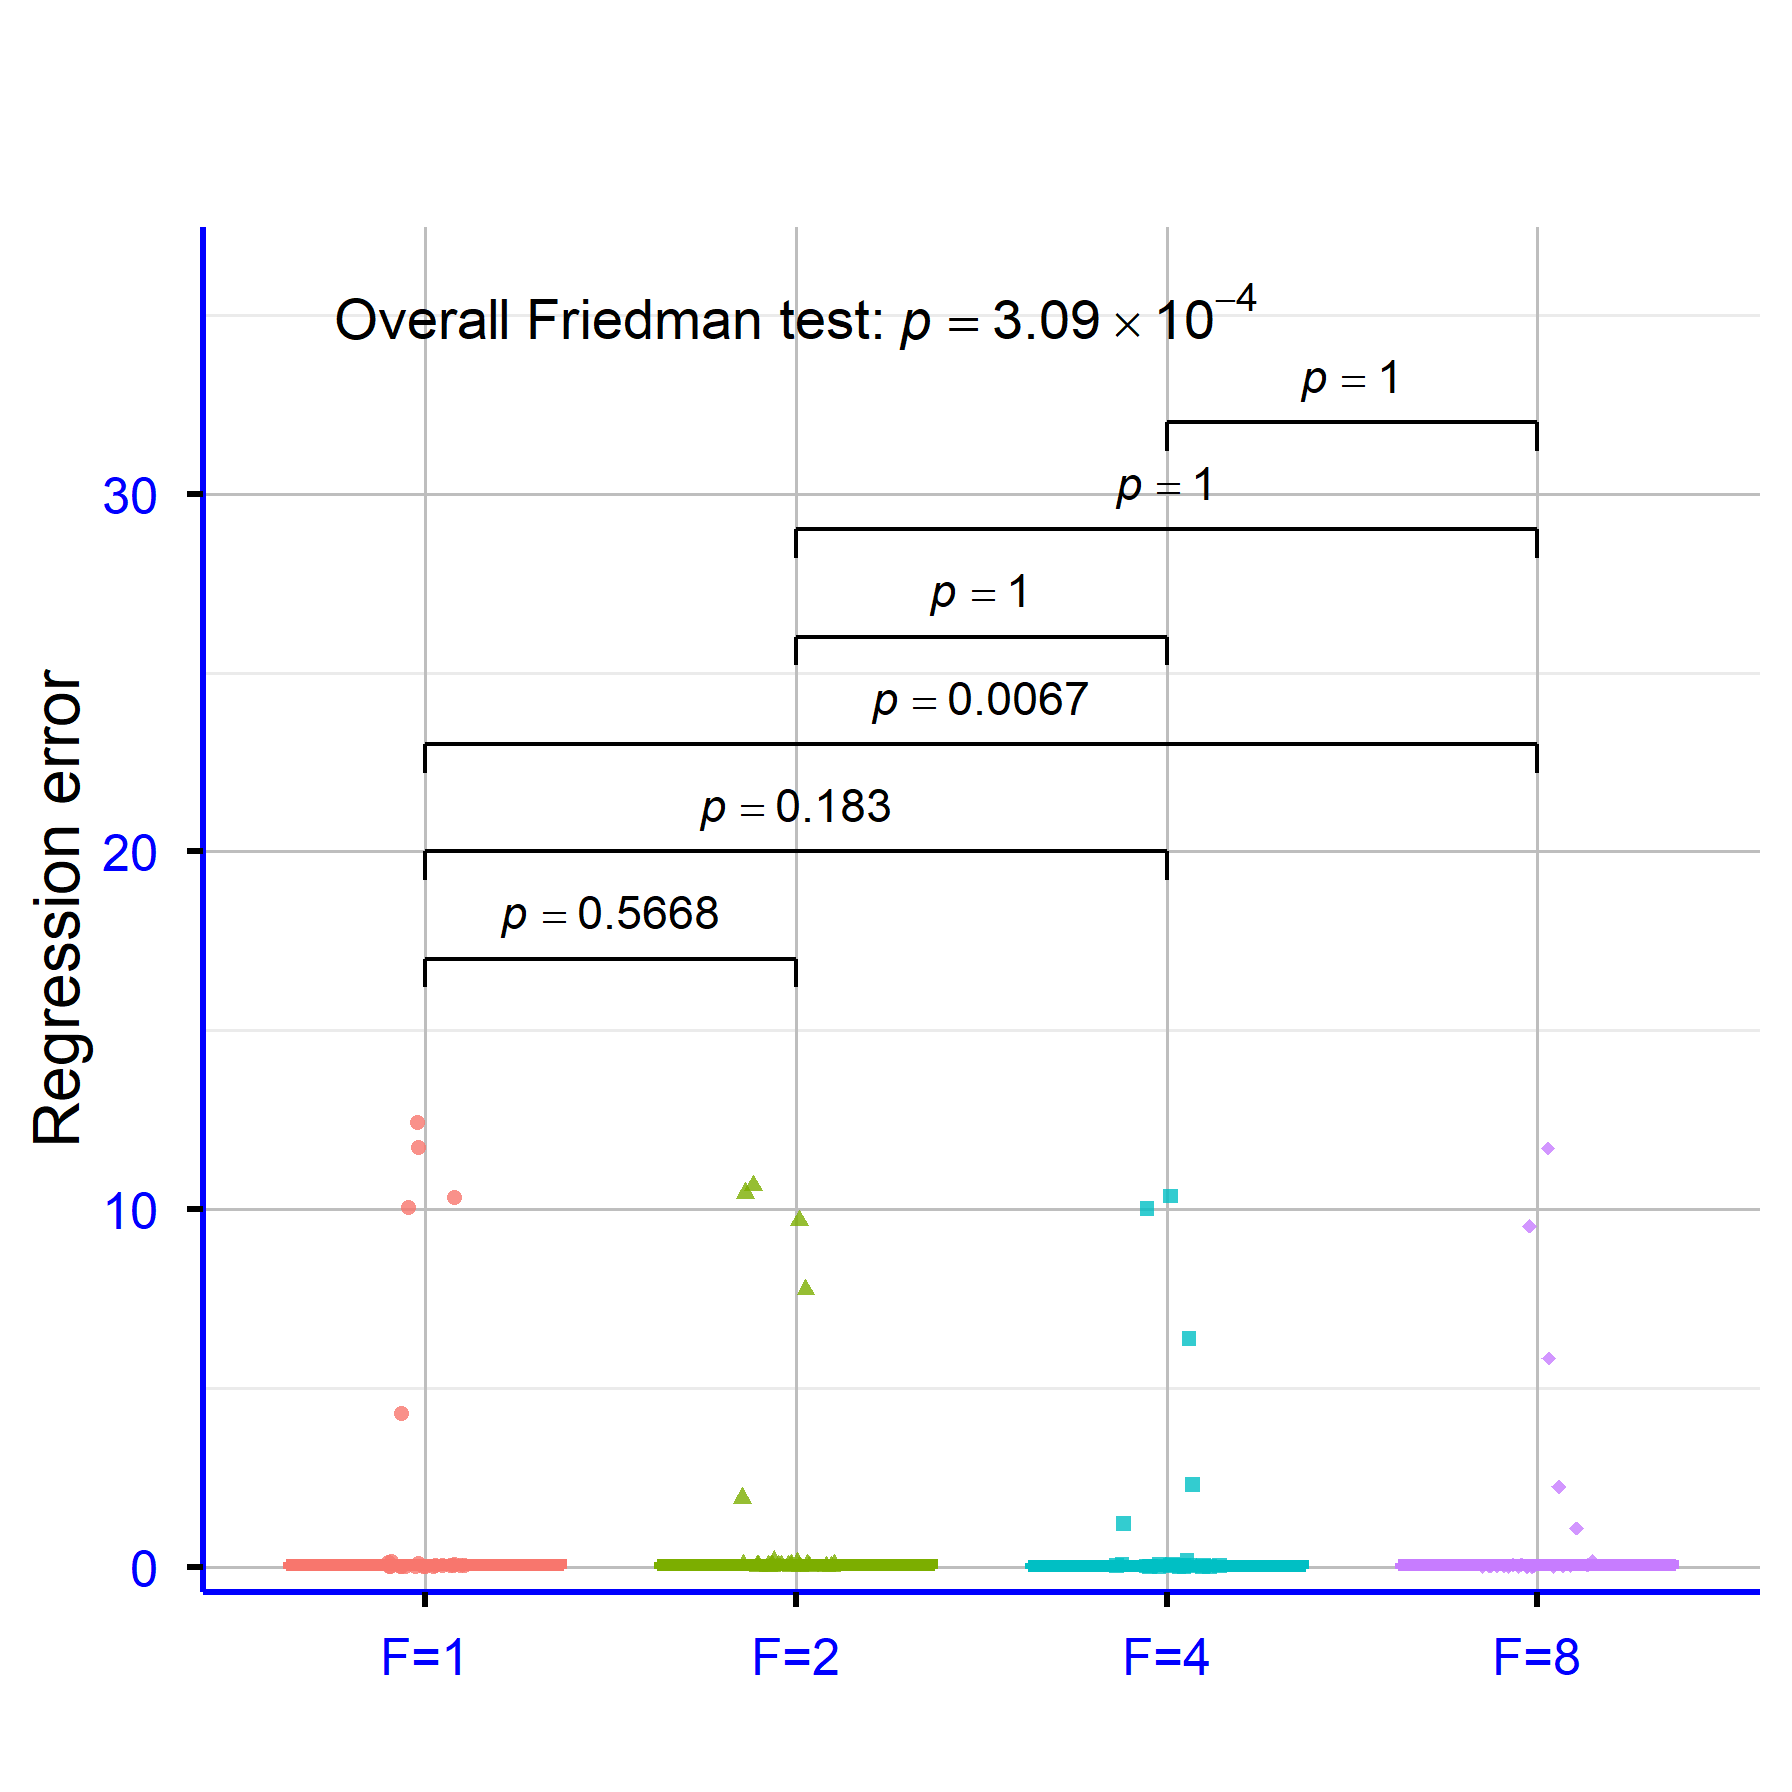
\includegraphics[scale=0.5]{stat_tbl5}
\par\end{centering}
\caption{Sensitivity of regression performance to the scale parameter F (overall
Friedman test: $p=9.06\times10^{-4}$).\label{fig:regressionF}}
\end{figure}


\subsection{Experiments with number of chromosomes $N_{c}$}

Table \ref{tab:experClassNc} and Figure \ref{fig:classNc} illustrate
the effect of the chromosome population size $N_{c}$ on classification
performance, while Table \ref{tab:experRegressionNC} and Figure \ref{fig:regressionNc}
present the corresponding regression results. For classification (Table
\ref{tab:experClassNc}), the mean error rates were 23.03\% for $N_{c}$=100,
22.44\% for $N_{c}$=200, 21.58\% for $N_{c}$=500, and 21.55\% for
$N_{c}$=1000. The overall Friedman test (Figure \ref{fig:classNc})
yielded p = 0.0037, confirming a statistically significant effect
of $N_{c}$ on classification accuracy. A steady improvement is observed
from $N_{c}$=100 to $N_{c}$=500, while the increase to $N_{c}$=1000
yields no meaningful additional gain, suggesting that a population
of 500 chromosomes offers a well-balanced trade-off between computational
cost and predictive performance. For regression (Table \ref{tab:experRegressionNC}),
the mean error values were 3.63 for $N_{c}$=100, 3.45 for $N_{c}$=200,
3.36 for $N_{c}$=500, and 3.55 for $N_{c}$=1000. The overall Friedman
test (Figure \ref{fig:regressionNc}) yielded $p=0.2415$, a value
that does not reach statistical significance, indicating that for
regression tasks the chromosome count does not substantially influence
performance and that $N_{c}$=500 remains a sufficient and well-justified
setting.

\begin{table}[H]
\caption{Experimental results on the classification datasets, using the proposed
method and different values the number of chromsosomes denoted as
$N_{c}$.\label{tab:experClassNc}}

\centering{}%
\begin{tabular}{|c|c|c|c|c|}
\hline 
DATASET & $N_{c}=100$ & $N_{c}=200$ & $N_{c}=500$ & $N_{c}=1000$\tabularnewline
\hline 
\hline 
APPENDICITIS & 20.00\% & 19.40\% & 17.80\% & 15.40\%\tabularnewline
\hline 
ALCOHOL & 25.32\% & 20.21\% & 20.43\% & 19.36\%\tabularnewline
\hline 
AUSTRALIAN & 23.87\% & 20.94\% & 18.90\% & 17.81\%\tabularnewline
\hline 
BALANCE & 17.18\% & 16.97\% & 17.50\% & 17.84\%\tabularnewline
\hline 
BANDS & 38.28\% & 36.61\% & 36.28\% & 36.17\%\tabularnewline
\hline 
CIRCULAR & 11.10\% & 6.42\% & 5.04\% & 5.29\%\tabularnewline
\hline 
CLEVELAND & 48.66\% & 48.86\% & 50.14\% & 50.38\%\tabularnewline
\hline 
DERMATOLOGY & 41.69\% & 41.94\% & 39.80\% & 40.83\%\tabularnewline
\hline 
ECOLI & 60.40\% & 60.76\% & 58.36\% & 59.52\%\tabularnewline
\hline 
FERT & 22.50\% & 21.10\% & 21.40\% & 24.00\%\tabularnewline
\hline 
GLASS & 55.99\% & 55.14\% & 52.76\% & 51.62\%\tabularnewline
\hline 
HABERMAN & 26.17\% & 26.77\% & 27.37\% & 27.53\%\tabularnewline
\hline 
HAYES ROTH & 41.61\% & 42.39\% & 40.08\% & 38.08\%\tabularnewline
\hline 
HEART & 22.85\% & 23.34\% & 22.00\% & 21.59\%\tabularnewline
\hline 
HEARTATTACK & 17.90\% & 18.87\% & 19.13\% & 18.83\%\tabularnewline
\hline 
HOUSEVOTES & 6.65\% & 6.35\% & 4.61\% & 5.35\%\tabularnewline
\hline 
IONOSPHERE & 14.66\% & 14.12\% & 12.83\% & 11.83\%\tabularnewline
\hline 
LIVERDISORDER & 29.50\% & 29.59\% & 30.41\% & 29.77\%\tabularnewline
\hline 
LYMOGRAPHY & 29.72\% & 29.79\% & 24.57\% & 22.43\%\tabularnewline
\hline 
MAMMOGRAPHIC & 18.27\% & 17.77\% & 17.72\% & 17.84\%\tabularnewline
\hline 
PARKINSONS & 15.95\% & 15.68\% & 15.53\% & 16.05\%\tabularnewline
\hline 
PAGE BLOCKS & 9.40\% & 9.36\% & 9.47\% & 10.43\%\tabularnewline
\hline 
PHONEME & 16.00\% & 15.54\% & 15.59\% & 16.37\%\tabularnewline
\hline 
PIMA & 23.50\% & 23.66\% & 23.59\% & 23.23\%\tabularnewline
\hline 
POPFAILURES & 5.91\% & 6.33\% & 5.61\% & 5.46\%\tabularnewline
\hline 
REGIONS2 & 25.71\% & 25.66\% & 25.71\% & 25.43\%\tabularnewline
\hline 
RING & 5.88\% & 5.88\% & 5.05\% & 4.46\%\tabularnewline
\hline 
SAHEART & 28.46\% & 28.00\% & 28.89\% & 28.94\%\tabularnewline
\hline 
SATIMAGE & 34.96\% & 35.21\% & 32.97\% & 35.15\%\tabularnewline
\hline 
SEGMENT & 33.05\% & 32.73\% & 32.47\% & 31.95\%\tabularnewline
\hline 
SONAR & 25.75\% & 25.00\% & 24.00\% & 22.95\%\tabularnewline
\hline 
SPAMBASE & 12.41\% & 11.74\% & 10.54\% & 10.11\%\tabularnewline
\hline 
SPIRAL & 40.59\% & 41.39\% & 41.03\% & 41.11\%\tabularnewline
\hline 
STATHEART & 23.78\% & 24.30\% & 23.89\% & 25.11\%\tabularnewline
\hline 
STUDENT & 22.18\% & 17.10\% & 12.43\% & 11.45\%\tabularnewline
\hline 
TRANSFUSION & 25.91\% & 25.74\% & 25.23\% & 25.34\%\tabularnewline
\hline 
WDBC & 4.54\% & 4.54\% & 4.19\% & 4.75\%\tabularnewline
\hline 
WINE & 11.00\% & 10.12\% & 10.59\% & 10.71\%\tabularnewline
\hline 
Z\_F\_S & 5.90\% & 5.43\% & 4.68\% & 6.07\%\tabularnewline
\hline 
ZO\_NF\_S & 7.74\% & 7.34\% & 5.47\% & 5.70\%\tabularnewline
\hline 
ZONF\_S & 3.26\% & 2.52\% & 1.82\% & 2.60\%\tabularnewline
\hline 
ZOO & 13.10\% & 11.90\% & 10.60\% & 10.40\%\tabularnewline
\hline 
\textbf{AVERAGE} & \textbf{23.03\%} & \textbf{22.44\%} & \textbf{21.58\%} & \textbf{21.55\%}\tabularnewline
\hline 
\end{tabular}
\end{table}

\begin{figure}[H]
\begin{centering}
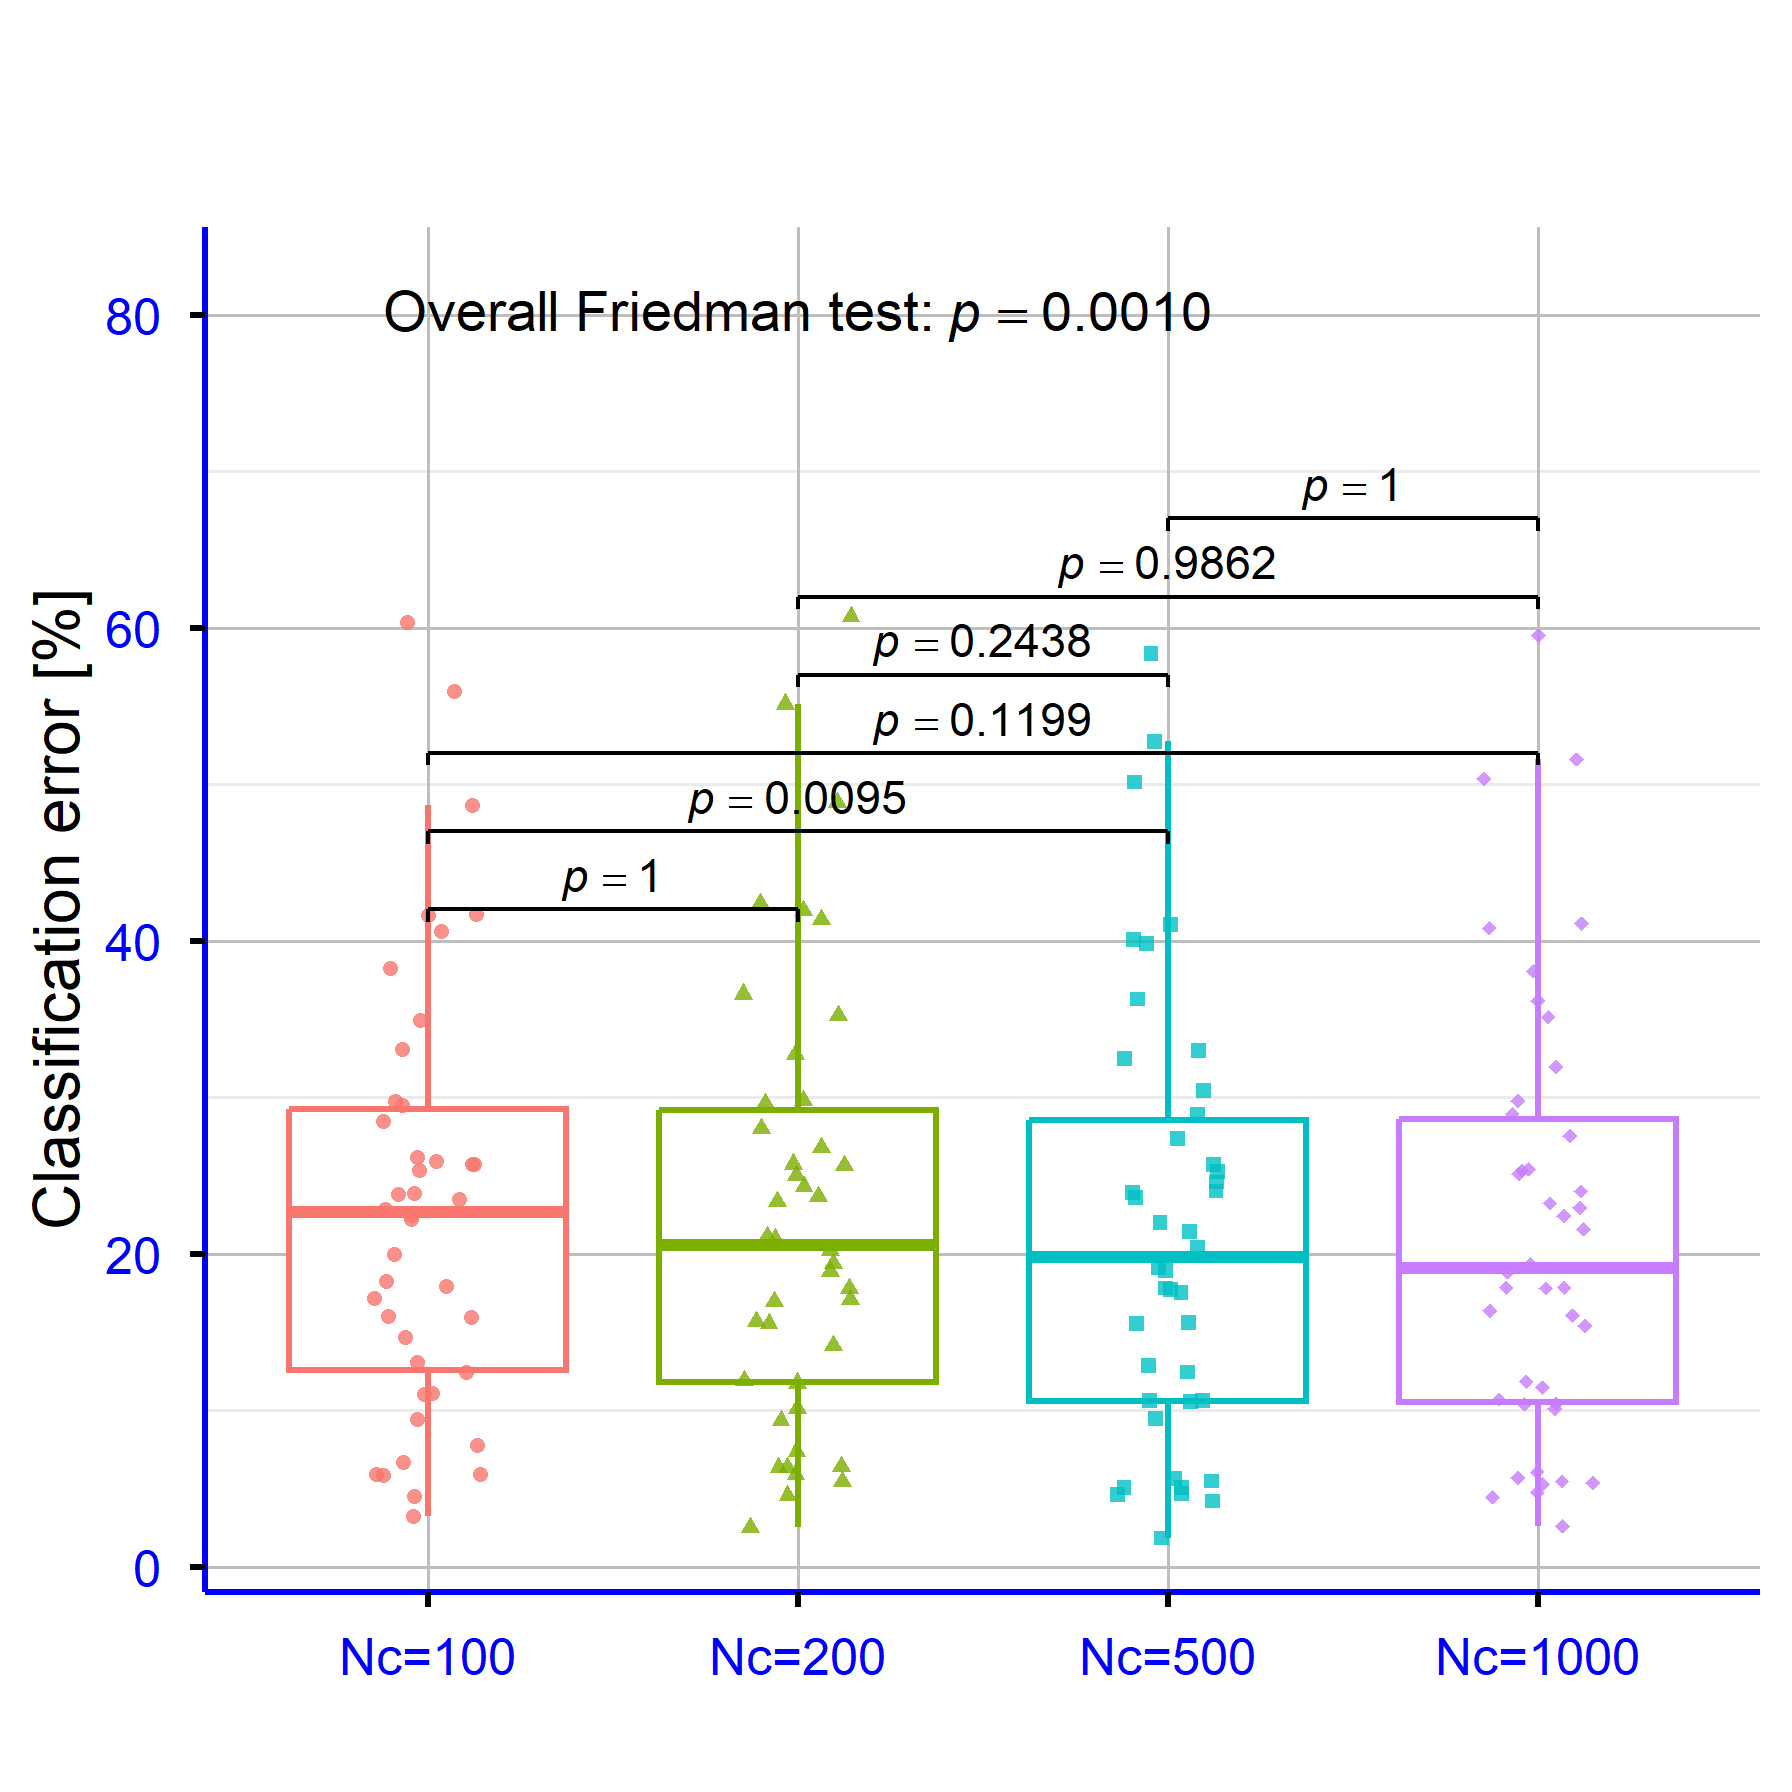
\includegraphics[scale=0.5]{stat_tbl6}
\par\end{centering}
\caption{Impact of population size Nc on classification results of the Proposed
method (overall Friedman test: $p=0.0037$).\label{fig:classNc}}
\end{figure}

\begin{table}[H]
\caption{Experimental results on the used regression datasets using the proposed
method and different values for the number of chromosomes $N_{c}$.\label{tab:experRegressionNC}}

\centering{}%
\begin{tabular}{|c|c|c|c|c|}
\hline 
DATASET & $N_{c}=100$ & $N_{c}=200$ & $N_{c}=500$ & $N_{c}=1000$\tabularnewline
\hline 
\hline 
ABALONE & 7.24 & 6.90 & 6.37 & 6.13\tabularnewline
\hline 
AIRFOIL & 0.004 & 0.004 & 0.004 & 0.004\tabularnewline
\hline 
AUTO & 9.70 & 9.57 & 10.02 & 9.88\tabularnewline
\hline 
BK & 0.02 & 0.02 & 0.021 & 0.022\tabularnewline
\hline 
BL & 0.0007 & 0.0006 & 0.0005 & 0.022\tabularnewline
\hline 
BASEBALL & 56.15 & 53.69 & 53.20 & 56.45\tabularnewline
\hline 
CONCRETE & 0.01 & 0.009 & 0.008 & 0.007\tabularnewline
\hline 
DEE & 0.23 & 0.16 & 0.16 & 0.16\tabularnewline
\hline 
FA & 0.025 & 0.022 & 0.019 & 0.016\tabularnewline
\hline 
FY & 0.049 & 0.049 & 0.051 & 0.051\tabularnewline
\hline 
HO & 0.007 & 0.007 & 0.007 & 0.008\tabularnewline
\hline 
HOUSING & 10.50 & 10.92 & 10.36 & 11.94\tabularnewline
\hline 
LASER & 0.058 & 0.025 & 0.0198 & 0.017\tabularnewline
\hline 
LW & 0.02 & 0.018 & 0.016 & 0.014\tabularnewline
\hline 
MB & 0.06 & 0.063 & 0.066 & 0.065\tabularnewline
\hline 
MORTGAGE & 0.014 & 0.008 & 0.0096 & 0.01\tabularnewline
\hline 
NT & 0.006 & 0.006 & 0.006 & 0.006\tabularnewline
\hline 
PLASTIC & 5.11 & 3.37 & 2.30 & 2.32\tabularnewline
\hline 
PY & 0.015 & 0.016 & 0.015 & 0.013\tabularnewline
\hline 
PL & 0.045 & 0.032 & 0.024 & 0.023\tabularnewline
\hline 
QUAKE & 0.036 & 0.036 & 0.036 & 0.036\tabularnewline
\hline 
SN & 0.023 & 0.023 & 0.024 & 0.024\tabularnewline
\hline 
STOCK & 1.31 & 1.22 & 1.208 & 1.38\tabularnewline
\hline 
TREASURY & 0.048 & 0.048 & 0.047 & 0.047\tabularnewline
\hline 
VE & 0.039 & 0.042 & 0.04 & 0.047\tabularnewline
\hline 
\textbf{AVERAGE} & \textbf{3.63} & \textbf{3.45} & \textbf{3.36} & \textbf{3.55}\tabularnewline
\hline 
\end{tabular}
\end{table}

\begin{figure}[H]
\begin{centering}
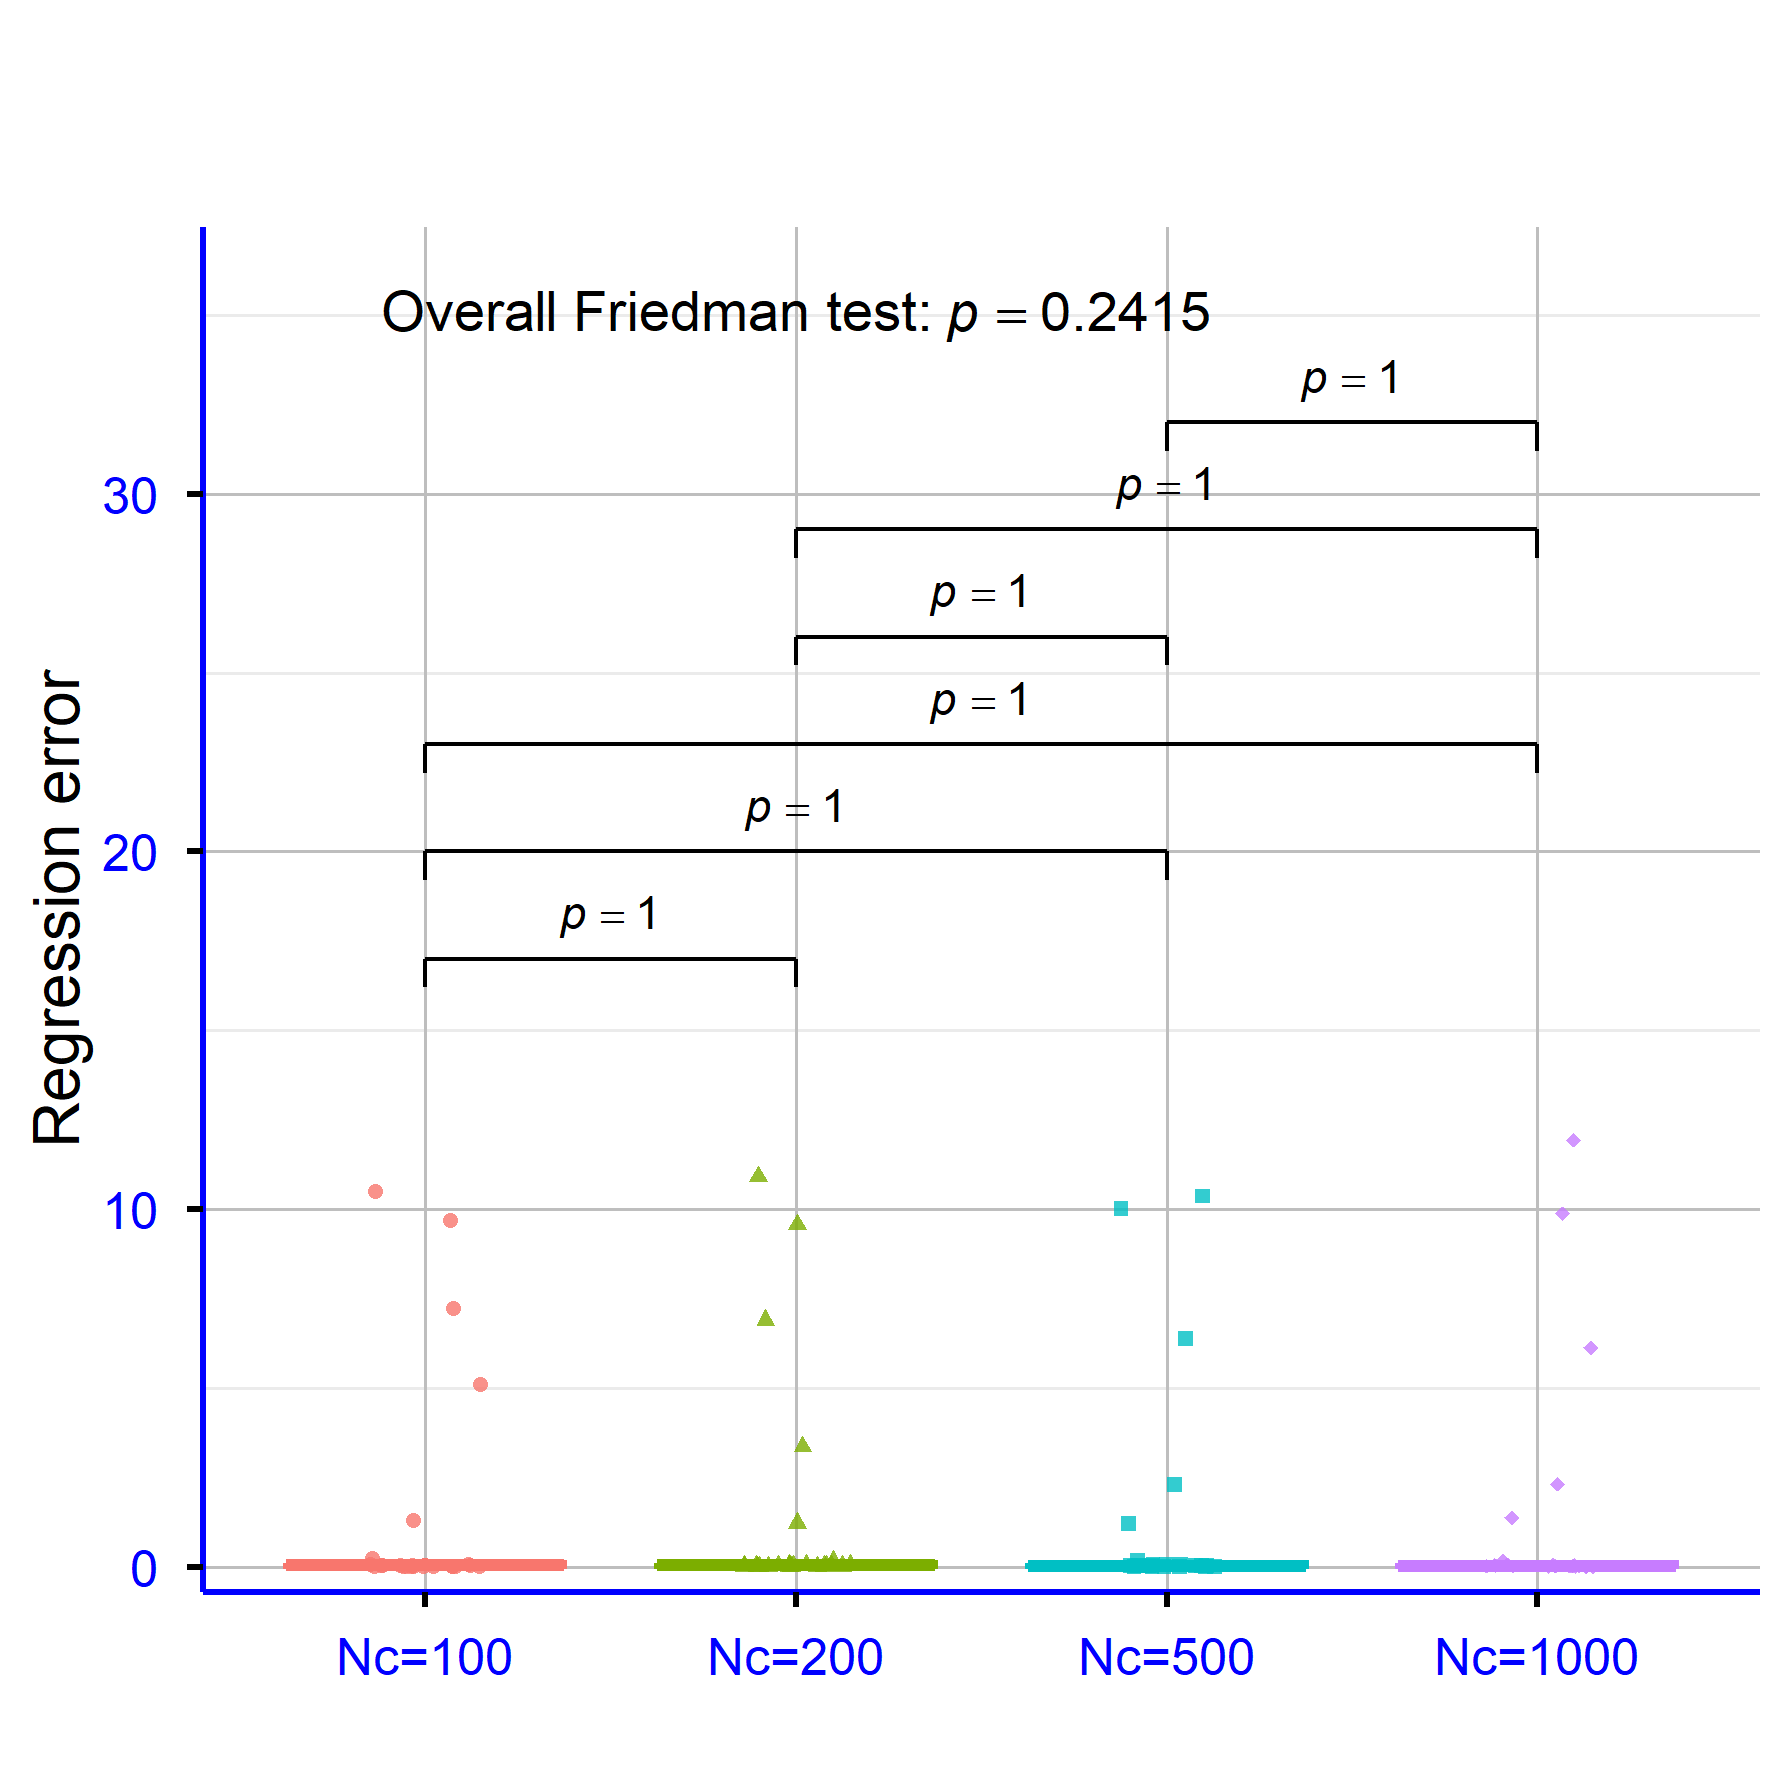
\includegraphics[scale=0.5]{stat_tbl7}
\par\end{centering}
\caption{Regression error under varying chromosome population sizes Nc (overall
Friedman test: $p=0.2415$).\label{fig:regressionNc}}
\end{figure}


\section{Conclusions\label{sec:Conclusions}}

This paper introduced a two-phase evolutionary methodology for the
effective training of Radial Basis Function networks. In the first
phase, the K-means clustering algorithm is employed to establish informed
search bounds for the network centers and variances, thereby constraining
the subsequent optimization within a meaningful parameter space. In
the second phase, a genetic algorithm operates within these bounds
to identify optimal center and variance configurations, while the
network weights are determined analytically by solving a system of
linear equations. The proposed method was evaluated across a large
and diverse collection of 42 classification and 25 regression benchmark
datasets, consistently outperforming five competing approaches, namely
ADAM, BFGS, NEAT, RBF, and GRBF. The mean classification error of
21.58\% and the mean regression error of 3.36 represent substantial
improvements over all baselines, and the differences were confirmed
to be statistically significant by the Friedman test. The sensitivity
analysis further demonstrated that the method is robust across a range
of parameter settings, with a population size of 500 chromosomes and
a scale factor of $F$=4 providing a reliable and computationally
efficient default configuration.

Several directions are proposed for future investigation. First, the
computational cost of the genetic algorithm could be reduced through
parallelization, enabling the simultaneous evaluation of multiple
candidate solutions across multi-core or distributed computing environments.
Second, adaptive strategies for the automatic selection of key parameters,
such as the population size $N_{c}$, the number of generations $N_{g}$,
and the scale factor $F$, could further reduce the need for manual
tuning while improving performance across diverse problem types. Third,
the current Gaussian basis function could be replaced or complemented
by alternative kernel functions, such as multiquadric or inverse multiquadric
kernels, potentially broadening the class of problems the model can
address effectively. Fourth, the integration of feature selection
mechanisms within the training pipeline could improve both accuracy
and interpretability, particularly for high-dimensional datasets.
Finally, extending the proposed framework to deep or multi-hidden-layer
RBF architectures represents a promising avenue for tackling more
complex learning tasks.

\vspace{6pt}


\authorcontributions{V.C. and I.G.T. conducted the experiments, employing several datasets
and provided the comparative experiments. D.T. and V.C. performed
the statistical analysis and prepared the manuscript. All authors
have read and agreed to the published version of the manuscript.}

\funding{This research has been financed by the European Union: Next Generation
EU through the Program Greece 2.0 National Recovery and Resilience
Plan, under the call RESEARCH---CREATE---INNOVATE, project name
“iCREW: Intelligent small craft simulator for advanced crew training
using Virtual Reality techniques” (project code:TAEDK-06195).}

\institutionalreview{Not applicable.}

\informedconsent{Not applicable.}

\dataavailability{The original contributions presented in this study are included in
the article. Further inquiries can be directed to the corresponding
author.}

\conflictsofinterest{The authors declare no conflicts of interest.}

\begin{adjustwidth}{-\extralength}{0cm}{}


\reftitle{References}
\begin{thebibliography}{999}
\bibitem[(2000)]{physics_ml1} Raissi, M., \& Karniadakis, G. E. (2018).
Hidden physics models: Machine learning of nonlinear partial differential
equations. Journal of Computational Physics, 357, 125-141.

\bibitem{physics_ml2}Kashinath, K., Mustafa, M., Albert, A., Wu,
J. L., Jiang, C., Esmaeilzadeh, S., ... \& Prabhat, N. (2021). Physics-informed
machine learning: case studies for weather and climate modelling.
Philosophical Transactions of the Royal Society A, 379(2194), 20200093.

\bibitem[(2006)]{astronomy_ml1}Viquar, M., Basak, S., Dasgupta, A.,
Agrawal, S., \& Saha, S. (2019). Machine learning in astronomy: A
case study in quasar-star classification. Emerging Technologies in
Data Mining and Information Security: Proceedings of IEMIS 2018, Volume
3, 827-836.

\bibitem[(2006)]{astronomy_ml2}Luo, S., Leung, A. P., Hui, C. Y.,
\& Li, K. L. (2020). An investigation on the factors affecting machine
learning classifications in gamma-ray astronomy. Monthly Notices of
the Royal Astronomical Society, 492(4), 5377-5390.

\bibitem[(2006)]{chemistry_ml1}Meuwly, M. (2021). Machine learning
for chemical reactions. Chemical Reviews, 121(16), 10218-10239.

\bibitem{chemistry_ml2}J.A. Aguiar, M.L. Gong, T.Tasdizen, Crystallographic
prediction from diffraction and chemistry data for higher throughput
classification using machine learning, Computational Materials Science
\textbf{173}, 109409, 2020.

\bibitem[(2006)]{med_ml1}S.S. Yadav, S.M. Jadhav, Deep convolutional
neural network based medical image classification for disease diagnosis.
J Big Data \textbf{6}, 113, 2019.

\bibitem{med_ml2}L. Qing, W. Linhong , D. Xuehai, A Novel Neural
Network-Based Method for Medical Text Classification, Future Internet
\textbf{11}, 255, 2019. 

\bibitem[(2006)]{econ_ml1}Athey, S. (2018). The impact of machine
learning on economics. In The economics of artificial intelligence:
An agenda (pp. 507-547). University of Chicago Press.

\bibitem{econ_ml2}R. Hafezi, J. Shahrabi, E. Hadavandi, A bat-neural
network multi-agent system (BNNMAS) for stock price prediction: Case
study of DAX stock price, Applied Soft Computing \textbf{29}, pp.
196-210, 2015.

\bibitem{nn_image}Ghai, D., Tripathi, S. L., Saxena, S., Chanda,
M., \& Alazab, M. (Eds.). (2022). Machine learning algorithms for
signal and image processing. John Wiley \& Sons.

\bibitem{nn_timeseries}Ahmed, N. K., Atiya, A. F., Gayar, N. E.,
\& El-Shishiny, H. (2010). An empirical comparison of machine learning
models for time series forecasting. Econometric reviews, 29(5-6),
594-621.

\bibitem[(2000)]{nn_credit}Z. Huang, H. Chen, C.-Jung Hsu, W.-Hwa
Chen, S. Wu, Credit rating analysis with support vector machines and
neural networks: a market comparative study, Decision Support Systems
\textbf{37}, pp. 543-558, 2004.

\bibitem{nn_mech1}K. Peta, J. Żurek, Prediction of air leakage in
heat exchangers for automotive applications using artificial neural
networks, In: 2018 9th IEEE Annual Ubiquitous Computing, Electronics
\& Mobile Communication Conference (UEMCON), New York, NY, USA, pp.
721-725, 2018.

\bibitem[(1991)]{rbf1}J. Park and I. W. Sandberg, Universal Approximation
Using Radial-Basis-Function Networks, Neural Computation \textbf{3},
pp. 246-257, 1991.

\bibitem{rbf2}G.A. Montazer, D. Giveki, M. Karami, H. Rastegar, Radial
basis function neural networks: A review. Comput. Rev. J \textbf{1},
pp. 52-74, 2018.

\bibitem[(2000)]{rbfphysics1}P. Teng, Machine-learning quantum mechanics:
Solving quantum mechanics problems using radial basis function networks,
Phys. Rev. E \textbf{98}, 033305, 2018.

\bibitem{rbfphysics2}R. Jovanović, A. Sretenovic, Ensemble of radial
basis neural networks with K-means clustering for heating energy consumption
prediction, FME Transactions \textbf{45}, pp. 51-57, 2017.

\bibitem{rbfphysics3}V.I. Gorbachenko, M.V. Zhukov, Solving boundary
value problems of mathematical physics using radial basis function
networks. Comput. Math. and Math. Phys. \textbf{57}, pp. 145--155,
2017.

\bibitem{rbfphysics4}J. Määttä, V. Bazaliy, J. Kimari, F. Djurabekova,
K. Nordlund, T. Roos, Gradient-based training and pruning of radial
basis function networks with an application in materials physics,
Neural Networks \textbf{133}, pp. 123-131, 2021.

\bibitem{rbfde1}Nam Mai-Duy, Thanh Tran-Cong, Numerical solution
of differential equations using multiquadric radial basis function
networks, Neural Networks 14, pp. 185-199, 2001.

\bibitem{rbfde2}N. Mai‐Duy, Solving high order ordinary differential
equations with radial basis function networks. Int. J. Numer. Meth.
Engng. \textbf{62}, pp. 824-852, 2005.

\bibitem{rbfde3}S.A. Sarra, Adaptive radial basis function methods
for time dependent partial differential equations, Applied Numerical
Mathematics \textbf{54}, pp. 79-94, 2005.

\bibitem{rbfrobotics1}R. -J. Lian, Adaptive Self-Organizing Fuzzy
Sliding-Mode Radial Basis-Function Neural-Network Controller for Robotic
Systems, IEEE Transactions on Industrial Electronics \textbf{61},
pp. 1493-1503, 2014.

\bibitem{rbfrobotics2}M. Vijay, D. Jena, Backstepping terminal sliding
mode control of robot manipulator using radial basis functional neural
networks. Computers \& Electrical Engineering \textbf{67}, pp. 690-707,
2018.

\bibitem{rbfface1}M.J. Er, S. Wu, J. Lu, H.L. Toh, Face recognition
with radial basis function (RBF) neural networks, IEEE Transactions
on Neural Networks \textbf{13}, pp. 697-710, 2002.

\bibitem{rbfnetwork1}C. Laoudias, P. Kemppi and C. G. Panayiotou,
Localization Using Radial Basis Function Networks and Signal Strength
Fingerprints in WLAN, GLOBECOM 2009 - 2009 IEEE Global Telecommunications
Conference, Honolulu, HI, 2009, pp. 1-6, 2009.

\bibitem{rbfnetwork2}M. Azarbad, S. Hakimi, A. Ebrahimzadeh, Automatic
recognition of digital communication signal, International journal
of energy, information and communications \textbf{3}, pp. 21-33, 2012.

\bibitem{rbfchemistry1}D.L. Yu, J.B. Gomm, D. Williams, Sensor fault
diagnosis in a chemical process via RBF neural networks, Control Engineering
Practice \textbf{7}, pp. 49-55, 1999.

\bibitem{rbfchemistry2}V. Shankar, G.B. Wright, A.L. Fogelson, R.M.
Kirby, A radial basis function (RBF) finite difference method for
the simulation of reaction--diffusion equations on stationary platelets
within the augmented forcing method, Int. J. Numer. Meth. Fluids \textbf{75},
pp. 1-22, 2014.

\bibitem{rbfecon0}W. Shen, X. Guo, C. Wu, D. Wu, Forecasting stock
indices using radial basis function neural networks optimized by artificial
fish swarm algorithm, Knowledge-Based Systems 24, pp. 378-385, 2011.

\bibitem{rbfecon1}J. A. Momoh, S. S. Reddy, Combined Economic and
Emission Dispatch using Radial Basis Function, 2014 IEEE PES General
Meeting \textbar{} Conference \& Exposition, National Harbor, MD,
pp. 1-5, 2014.

\bibitem{rbfecon2}P. Sohrabi, B. Jodeiri Shokri, H. Dehghani, Predicting
coal price using time series methods and combination of radial basis
function (RBF) neural network with time series. Miner Econ 2021.

\bibitem{rbf_dos1}U. Ravale, N. Marathe, P. Padiya, Feature Selection
Based Hybrid Anomaly Intrusion Detection System Using K Means and
RBF Kernel Function, Procedia Computer Science \textbf{45}, pp. 428-435,
2015.

\bibitem{rbf_dos2}M. Lopez-Martin, A. Sanchez-Esguevillas, J. I.
Arribas, B. Carro, Network Intrusion Detection Based on Extended RBF
Neural Network With Offline Reinforcement Learning, IEEE Access \textbf{9},
pp. 153153-153170, 2021.

\bibitem[(2006)]{rbf_time}Gan, M., Peng, H., \& Dong, X. P. (2012).
A hybrid algorithm to optimize RBF network architecture and parameters
for nonlinear time series prediction. Applied Mathematical Modelling,
36(7), 2911-2919.

\bibitem[(2006)]{rbf_wind}G. Sideratos and N. Hatziargyriou, \textquotedbl Using
Radial Basis Neural Networks to Estimate Wind Power Production,\textquotedbl{}
2007 IEEE Power Engineering Society General Meeting, Tampa, FL, USA,
2007, pp. 1-7, doi: 10.1109/PES.2007.385812.

\bibitem{rbfinit1}L.I. Kuncheva, Initializing of an RBF network by
a genetic algorithm, Neurocomputing \textbf{14}, pp. 273-288, 1997.

\bibitem{rbfinit2}F. Ros, M. Pintore, A. Deman, J.R. Chrétien, Automatical
initialization of RBF neural networks, Chemometrics and Intelligent
Laboratory Systems \textbf{87}, pp. 26-32, 2007.

\bibitem{rbfinit3}D. Wang, X.J. Zeng, J.A. Keane, A clustering algorithm
for radial basis function neural network initialization, Neurocomputing
\textbf{77}, pp. 144-155, 2012.

\bibitem{rbfkernel}N. Benoudjit, M. Verleysen, On the Kernel Widths
in Radial-Basis Function Networks, Neural Processing Letters \textbf{18},
pp. 139--154, 2003.

\bibitem{rbflearn}R. Neruda, P. Kudova, Learning methods for radial
basis function networks, Future Generation Computer Systems \textbf{21},
pp. 1131--1142, 2005.

\bibitem{rbfprun1}E. Ricci, R. Perfetti, Improved pruning strategy
for radial basis function networks with dynamic decay adjustment,
Neurocomputing \textbf{69}, pp. 1728-1732, 2006.

\bibitem{rbfprun3}Guang-Bin Huang, P. Saratchandran and N. Sundararajan,
A generalized growing and pruning RBF (GGAP-RBF) neural network for
function approximation, IEEE Transactions on Neural Networks \textbf{16},
pp. 57-67, 2005.

\bibitem{rbfprun2}M. Bortman and M. Aladjem, A Growing and Pruning
Method for Radial Basis Function Networks, IEEE Transactions on Neural
Networks \textbf{20}, pp. 1039-1045, 2009.

\bibitem{rbfpar1}R. Yokota, L.A. Barba, M. G. Knepley, PetRBF ---
A parallel O(N) algorithm for radial basis function interpolation
with Gaussians, Computer Methods in Applied Mechanics and Engineering
\textbf{199}, pp. 1793-1804, 2010.

\bibitem{rbfpar2}C. Lu, N. Ma, Z. Wang, Fault detection for hydraulic
pump based on chaotic parallel RBF network, EURASIP J. Adv. Signal
Process. \textbf{2011}, 49, 2011.

\bibitem[(2006)]{rbf_universal}J. Park and I. W. Sandberg, \textquotedbl Universal
Approximation Using Radial-Basis-Function Networks,\textquotedbl{}
in Neural Computation, vol. 3, no. 2, pp. 246-257, June 1991, doi:
\url{10.1162/neco.1991.3.2.246}. 

\bibitem[(2000)]{kmeans}E.U. Oti, M.O. Olusola, F.C. Eze, S.U. Enogwe,
Comprehensive review of K-Means clustering algorithms, Criterion \textbf{12},
pp. 22-23, 2021.

\bibitem{ga1}D. Goldberg, Genetic Algorithms in Search, Optimization
and Machine Learning, Addison-Wesley Publishing Company, Reading,
Massachussets, 1989.

\bibitem{ga2}Z. Michaelewicz, Genetic Algorithms + Data Structures
= Evolution Programs. Springer - Verlag, Berlin, 1996.

\bibitem{gen_app1}S.A. Grady, M.Y. Hussaini, M.M. Abdullah, Placement
of wind turbines using genetic algorithms, Renewable Energy \textbf{30},
pp. 259-270, 2005.

\bibitem{gen_app2}Parvaze, S., Kumar, R., Khan, J. N., Al-Ansari,
N., Parvaze, S., Vishwakarma, D. K., ... \& Kuriqi, A. (2023). Optimization
of water distribution systems using genetic algorithms: A review.
Archives of Computational Methods in Engineering, 30(7), 4209-4244.

\bibitem{gen_app3}Gordini, N. (2014). A genetic algorithm approach
for SMEs bankruptcy prediction: Empirical evidence from Italy. Expert
systems with applications, 41(14), 6433-6445.

\bibitem{gen_app4}Ding, S., Su, C., \& Yu, J. (2011). An optimizing
BP neural network algorithm based on genetic algorithm. Artificial
intelligence review, 36(2), 153-162.

\bibitem[(2000)]{kaelo}P. Kaelo, M.M. Ali, Integrated crossover rules
in real coded genetic algorithms, European Journal of Operational
Research \textbf{176}, pp. 60-76, 2007.

\bibitem[(2004)]{powell}M.J.D Powell, A Tolerant Algorithm for Linearly
Constrained Optimization Calculations, Mathematical Programming \textbf{45},
pp. 547-566, 1989. 

\bibitem[(1989)]{uci} M. Kelly, R. Longjohn, K. Nottingham, The UCI
Machine Learning Repository, \url{https://archive.ics.uci.edu}.

\bibitem{Keel}J. Alcalá-Fdez, A. Fernandez, J. Luengo, J. Derrac,
S. García, L. Sánchez, F. Herrera. KEEL Data-Mining Software Tool:
Data Set Repository, Integration of Algorithms and Experimental Analysis
Framework. Journal of Multiple-Valued Logic and Soft Computing 17,
pp. 255-287, 2011.

\bibitem{appendicitis}Weiss, Sholom M. and Kulikowski, Casimir A.,
Computer Systems That Learn: Classification and Prediction Methods
from Statistics, Neural Nets, Machine Learning, and Expert Systems,
Morgan Kaufmann Publishers Inc, 1991.

\bibitem[Tzimourta(2018)]{alcohol}Tzimourta, K.D.; Tsoulos, I.; Bilero,
I.T.; Tzallas, A.T.; Tsipouras, M.G.; Giannakeas, N. Direct Assessment
of Alcohol Consumption in Mental State Using Brain Computer Interfaces
and Grammatical Evolution. Inventions 2018, 3, 51.

\bibitem{australian}J.R. Quinlan, Simplifying Decision Trees. International
Journal of Man-Machine Studies \textbf{27}, pp. 221-234, 1987. 

\bibitem{balance}T. Shultz, D. Mareschal, W. Schmidt, Modeling Cognitive
Development on Balance Scale Phenomena, Machine Learning \textbf{16},
pp. 59-88, 1994.

\bibitem{Bands}B. Evans, D. Fisher, Overcoming process delays with
decision tree induction, IEEE Expert \textbf{9}, pp. 60-66, 1994.

\bibitem{cleveland1}Z.H. Zhou,Y. Jiang, NeC4.5: neural ensemble based
C4.5,\textquotedbl{} in IEEE Transactions on Knowledge and Data Engineering
\textbf{16}, pp. 770-773, 2004.

\bibitem{cleveland2}R. Setiono , W.K. Leow, FERNN: An Algorithm for
Fast Extraction of Rules from Neural Networks, Applied Intelligence
\textbf{12}, pp. 15-25, 2000.

\bibitem{dermatology}G. Demiroz, H.A. Govenir, N. Ilter, Learning
Differential Diagnosis of Eryhemato-Squamous Diseases using Voting
Feature Intervals, Artificial Intelligence in Medicine. \textbf{13},
pp. 147--165, 1998.

\bibitem[(1996)]{ecoli}P. Horton, K.Nakai, A Probabilistic Classification
System for Predicting the Cellular Localization Sites of Proteins,
In: Proceedings of International Conference on Intelligent Systems
for Molecular Biology \textbf{4}, pp. 109-15, 1996.

\bibitem{hayesroth}B. Hayes-Roth, B., F. Hayes-Roth. Concept learning
and the recognition and classification of exemplars. Journal of Verbal
Learning and Verbal Behavior \textbf{16}, pp. 321-338, 1977.

\bibitem{heart}I. Kononenko, E. Šimec, M. Robnik-Šikonja, Overcoming
the Myopia of Inductive Learning Algorithms with RELIEFF, Applied
Intelligence \textbf{7}, pp. 39--55, 1997

\bibitem{housevotes}R.M. French, N. Chater, Using noise to compute
error surfaces in connectionist networks: a novel means of reducing
catastrophic forgetting, Neural Comput. \textbf{14}, pp. 1755-1769,
2002.

\bibitem{ion1}J.G. Dy , C.E. Brodley, Feature Selection for Unsupervised
Learning, The Journal of Machine Learning Research \textbf{5}, pp
845--889, 2004.

\bibitem{ion2}S. J. Perantonis, V. Virvilis, Input Feature Extraction
for Multilayered Perceptrons Using Supervised Principal Component
Analysis, Neural Processing Letters \textbf{10}, pp 243--252, 1999.

\bibitem{liver} J. Garcke, M. Griebel, Classification with sparse
grids using simplicial basis functions, Intell. Data Anal. \textbf{6},
pp. 483-502, 2002.

\bibitem[(2002)]{lymography}G. Cestnik, I. Konenenko, I. Bratko,
Assistant-86: A Knowledge-Elicitation Tool for Sophisticated Users.
In: Bratko, I. and Lavrac, N., Eds., Progress in Machine Learning,
Sigma Press, Wilmslow, pp. 31-45, 1987. 

\bibitem{mammographic}M. Elter, R. Schulz-Wendtland, T. Wittenberg,
The prediction of breast cancer biopsy outcomes using two CAD approaches
that both emphasize an intelligible decision process, Med Phys. \textbf{34},
pp. 4164-72, 2007.

\bibitem{parkinsons}Little MA, McSharry PE, Hunter EJ, Spielman J,
Ramig LO. Suitability of dysphonia measurements for telemonitoring
of Parkinson's disease. IEEE Trans Biomed Eng. 2009;56(4):1015. doi:10.1109/TBME.2008.2005954

\bibitem{pima}J.W. Smith, J.E. Everhart, W.C. Dickson, W.C. Knowler,
R.S. Johannes, Using the ADAP learning algorithm to forecast the onset
of diabetes mellitus, In: Proceedings of the Symposium on Computer
Applications and Medical Care IEEE Computer Society Press, pp.261-265,
1988.

\bibitem{popfailures}D.D. Lucas, R. Klein, J. Tannahill, D. Ivanova,
S. Brandon, D. Domyancic, Y. Zhang, Failure analysis of parameter-induced
simulation crashes in climate models, Geoscientific Model Development
\textbf{6}, pp. 1157-1171, 2013.

\bibitem{regions}Giannakeas, N., Tsipouras, M.G., Tzallas, A.T.,
Kyriakidi, K., Tsianou, Z.E., Manousou, P., Hall, A., Karvounis, E.C.,
Tsianos, V., Tsianos, E. A clustering based method for collagen proportional
area extraction in liver biopsy images (2015) Proceedings of the Annual
International Conference of the IEEE Engineering in Medicine and Biology
Society, EMBS, 2015-November, art. no. 7319047, pp. 3097-3100. 

\bibitem{saheart}T. Hastie, R. Tibshirani, Non-parametric logistic
and proportional odds regression, JRSS-C (Applied Statistics) \textbf{36},
pp. 260--276, 1987.

\bibitem{segment}M. Dash, H. Liu, P. Scheuermann, K. L. Tan, Fast
hierarchical clustering and its validation, Data \& Knowledge Engineering
\textbf{44}, pp 109--138, 2003.

\bibitem[(1988)]{sonar}Gorman, R.P.; Sejnowski, T.J. Analysis of
Hidden Units in a Layered Network Trained to Classify Sonar Targets.
Neural Netw. 1988, 1, 75--89.

\bibitem[(2000)]{spambase}Cranor, Lorrie F., LaMacchia, Brian A.
Spam!, Communications of the ACM, 41(8):74-83, 1998.

\bibitem[(2007)]{student}P. Cortez, A. M. Gonçalves Silva, Using
data mining to predict secondary school student performance, In Proceedings
of 5th FUture BUsiness TEChnology Conference (FUBUTEC 2008) (pp. 5--12).
EUROSIS-ETI, 2008.

\bibitem[(2007)]{transfusion}I-Cheng Yeh, King-Jang Yang, Tao-Ming
Ting, Knowledge discovery on RFM model using Bernoulli sequence, Expert
Systems with Applications \textbf{36}, pp. 5866-5871, 2009.

\bibitem{wdbc}W.H. Wolberg, O.L. Mangasarian, Multisurface method
of pattern separation for medical diagnosis applied to breast cytology,
Proc Natl Acad Sci U S A. \textbf{87}, pp. 9193--9196, 1990.

\bibitem{wine1}M. Raymer, T.E. Doom, L.A. Kuhn, W.F. Punch, Knowledge
discovery in medical and biological datasets using a hybrid Bayes
classifier/evolutionary algorithm. IEEE transactions on systems, man,
and cybernetics. Part B, Cybernetics : a publication of the IEEE Systems,
Man, and Cybernetics Society, \textbf{33} , pp. 802-813, 2003.

\bibitem{wine2}P. Zhong, M. Fukushima, Regularized nonsmooth Newton
method for multi-class support vector machines, Optimization Methods
and Software \textbf{22}, pp. 225-236, 2007.

\bibitem{eeg}R.G. Andrzejak, K. Lehnertz, F. Mormann, C. Rieke, P.
David, and C. E. Elger, Indications of nonlinear deterministic and
finite-dimensional structures in time series of brain electrical activity:
Dependence on recording region and brain state, Phys. Rev. E \textbf{64},
pp. 1-8, 2001.

\bibitem{zoo}M. Koivisto, K. Sood, Exact Bayesian Structure Discovery
in Bayesian Networks, The Journal of Machine Learning Research\textbf{
5}, pp. 549--573, 2004.

\bibitem{abalone}W. J Nash, T.L. Sellers, S.R. Talbot, A.J. Cawthor,
W.B. Ford, The Population Biology of Abalone (\_Haliotis\_ species)
in Tasmania. I. Blacklip Abalone (\_H. rubra\_) from the North Coast
and Islands of Bass Strait, Sea Fisheries Division, Technical Report
No. 48 (ISSN 1034-3288), 1994.

\bibitem{airfoil}T.F. Brooks, D.S. Pope, and A.M. Marcolini. Airfoil
self-noise and prediction. Technical report, NASA RP-1218, July 1989. 

\bibitem{Stat}J.S. Simonoff, Smooting Methods in Statistics, Springer
- Verlag, 1996.

\bibitem{concrete}I.Cheng Yeh, Modeling of strength of high performance
concrete using artificial neural networks, Cement and Concrete Research.
\textbf{28}, pp. 1797-1808, 1998. 

\bibitem[(2007)]{housing}D. Harrison and D.L. Rubinfeld, Hedonic
prices and the demand for clean ai, J. Environ. Economics \& Management
\textbf{5}, pp. 81-102, 1978.

\bibitem{key21}J.S. Simonoff, Smooting Methods in Statistics, Springer
- Verlag, 1996.

\bibitem{ntdataset}Mackowiak, P.A., Wasserman, S.S., Levine, M.M.,
1992. A critical appraisal of 98.6 degrees f, the upper limit of the
normal body temperature, and other legacies of Carl Reinhold August
Wunderlich. J. Amer. Med. Assoc. 268, 1578--1580

\bibitem{pydataset}R.D. King, S. Muggleton, R. Lewis, M.J.E. Sternberg,
Proc. Nat. Acad. Sci. USA \textbf{89}, pp. 11322--11326, 1992. 

\bibitem{quake}M. Sikora, L. Wrobel, Application of rule induction
algorithms for analysis of data collected by seismic hazard monitoring
systems in coal mines, Archives of Mining Sciences \textbf{55}, pp.
91-114, 2010.

\bibitem[(2022)]{optimus}Tsoulos, I. G., Charilogis, V., Kyrou, G.,
Stavrou, V. N., \& Tzallas, A. (2025). OPTIMUS: A Multidimensional
Global Optimization Package. Journal of Open Source Software, 10(108),
7584.

\bibitem[(2016)]{armadillo}Sanderson, C., \& Curtin, R. (2016). Armadillo:
a template-based C++ library for linear algebra. The Journal of Open
Source Software, 1(2), 26-26.

\bibitem[(2016)]{adept}Hogan, R. J. Adept C++ Software Library: User
Guide.

\bibitem[(2025)]{bfgs}Yuan, Y. X. (1991). A modified BFGS algorithm
for unconstrained optimization. IMA Journal of Numerical Analysis,
11(3), 325-332.

\bibitem{nn1}C. Bishop, Neural Networks for Pattern Recognition,
Oxford University Press, 1995.

\bibitem{nn2}G. Cybenko, Approximation by superpositions of a sigmoidal
function, Mathematics of Control Signals and Systems \textbf{2}, pp.
303-314, 1989.

\bibitem{Adam}D. P. Kingma, J. L. Ba, ADAM: a method for stochastic
optimization, in: Proceedings of the 3rd International Conference
on Learning Representations (ICLR 2015), pp. 1--15, 2015.

\bibitem{AdamNN}Y. Xue, Y. Tong, F. Neri, An ensemble of differential
evolution and Adam for training feed-forward neural networks. Information
Sciences \textbf{608}, pp. 453-471, 2022.

\bibitem[(2025)]{neat}K. O. Stanley, R. Miikkulainen, Evolving Neural
Networks through Augmenting Topologies, Evolutionary Computation \textbf{10},
pp. 99-127, 2002.

\bibitem[(2016)]{genrbf}S. Ding, L. Xu, C. Su et al, An optimizing
method of RBF neural network based on genetic algorithm. Neural Comput
\& Applic 21, pp. 333--336, 2012.

\end{thebibliography}
%%%%%%%%%%%%%%%%%%%%%%%%%%%%%%%%%%%%%%%%%%
%% for journal Sci
%\reviewreports{\\
%Reviewer 1 comments and authors' response\\
%Reviewer 2 comments and authors' response\\
%Reviewer 3 comments and authors' response
%}
%%%%%%%%%%%%%%%%%%%%%%%%%%%%%%%%%%%%%%%%%%

\PublishersNote{}

\end{adjustwidth}{}
\end{document}
